\documentclass[12pt,prd]{article}
\pdfoutput=1
\usepackage{jheppub}
\usepackage{rotating}
\usepackage{array}
\usepackage{amsmath}
\usepackage[normalem]{ulem}
\usepackage{slashed}
\usepackage{booktabs}
\usepackage[pdftex,table]{xcolor}
\usepackage{units}
\usepackage{xfrac}
\usepackage{mathtools}
\usepackage{empheq}
\usepackage[]{units}
\usepackage{multirow}
\usepackage{amssymb}
\usepackage{url}
\usepackage{comment}
\usepackage{paralist}
\usepackage{caption}
\usepackage{forloop}

\usepackage{tikz}
\newcommand*\widefbox[1]{\fbox{\hspace{2em}#1\hspace{2em}}}

\def\beq{\begin{equation}}
\def\eeq{\end{equation}}
\newcommand{\bea}{\begin{eqnarray}\begin{aligned}}
\newcommand{\eea}{\end{aligned}\end{eqnarray}}
\def\bitem{\begin{itemize}}
\def\eitem{\end{itemize}}

 \widowpenalty10000 
 \clubpenalty10000


\usepackage{lineno}
\linenumbers

\abstract{
Blah
}

\keywords{}

\begin{document}
\title{CWoLas in Space}

\author[1]{Sowmya,} 
\author[2]{Benjamin Nachman,}
\author[3]{David Shih,}
\author[5]{others,}

\affiliation[2]{\normalsize Physics Division, Lawrence Berkeley National Laboratory, Berkeley, CA 94720, USA}
\affiliation[3]{\normalsize NHETC, Department of Physics and Astronomy, Rutgers University, Piscataway, NJ 08854, USA}

\emailAdd{bpnachman@lbl.gov}
\emailAdd{shih@physics.rutgers.edu}

\maketitle

 %===================================================================
\section{Introduction}\label{sec:intro}
%===================================================================

 %===================================================================
\section{Results}\label{sec:results}
%===================================================================

\newcounter{imagenum}
\begin{figure}[h!]
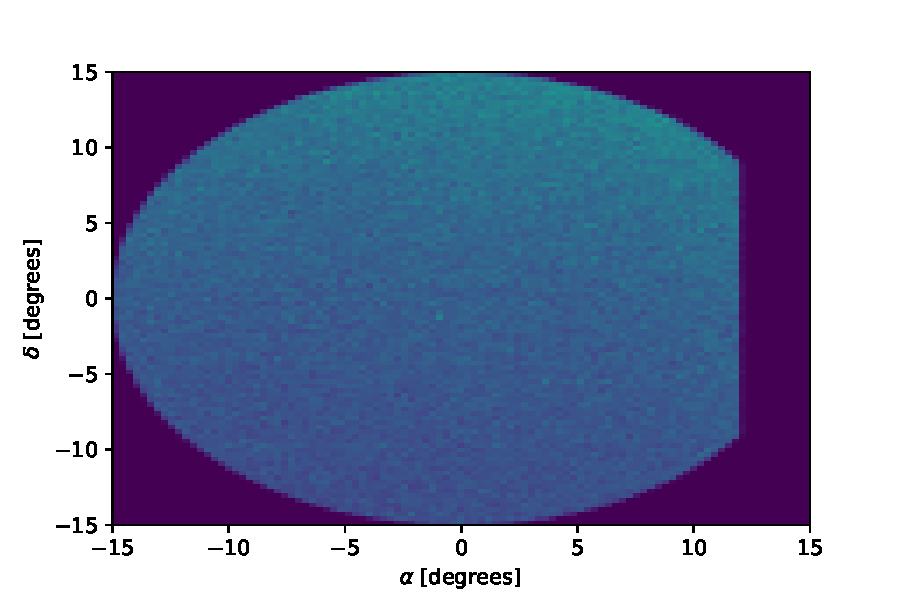
\includegraphics[width=0.5\textwidth]{../figures/histogram2dgaiascan_l101_2_b58_4_ra212_7_dec55_2_npy.pdf}\forloop{imagenum}{0}{\value{imagenum} < 18}{
\includegraphics[width=0.24\textwidth]{../figures/scanning_plotsgaiascan_l101_2_b58_4_ra212_7_dec55_2_npy_\arabic{imagenum}.pdf}}
\caption{Region l$101.2$ b$58.4$ ra$212.7$ dec$55.2$}
\end{figure}

\begin{figure}[h!]
\centering
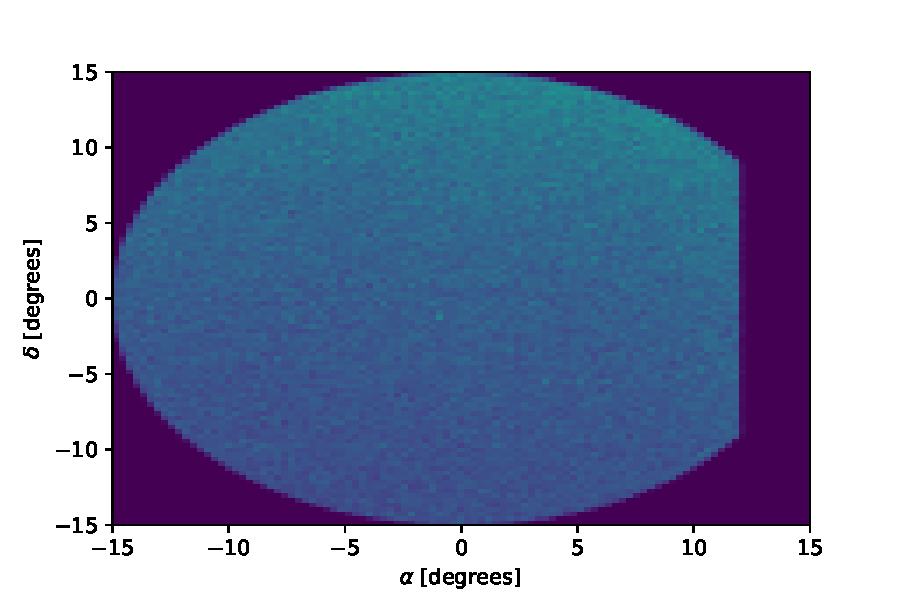
\includegraphics[width=0.5\textwidth]{../figures/histogram2dgaiascan_l101_2_b58_4_ra212_7_dec55_2_npy.pdf}\forloop{imagenum}{0}{\value{imagenum} < 18}{
\includegraphics[width=0.24\textwidth]{../figures/stars_near_zero_2dhistgaiascan_l101_2_b58_4_ra212_7_dec55_2_npy_\arabic{imagenum}.pdf}}
\caption{Stars near zero at Region l$101.2$ b$58.4$ ra$212.7$ dec$55.2$}
\end{figure}

\begin{figure}[h!]
\centering
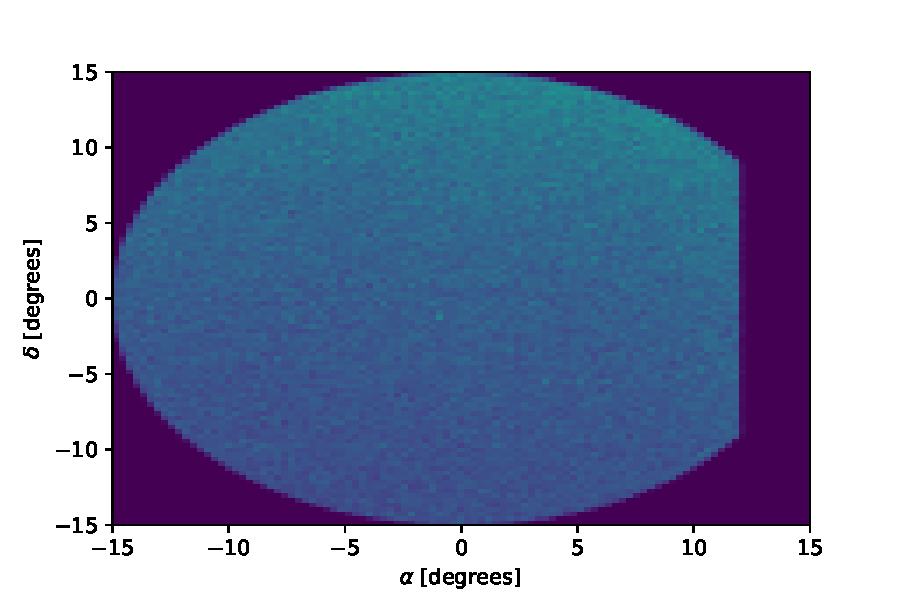
\includegraphics[width=0.5\textwidth]{../figures/histogram2dgaiascan_l101_2_b58_4_ra212_7_dec55_2_npy.pdf}\forloop{imagenum}{0}{\value{imagenum} < 18}{
\includegraphics[width=0.24\textwidth]{../figures/stars_near_zero_rahistgaiascan_l101_2_b58_4_ra212_7_dec55_2_npy_\arabic{imagenum}.pdf}}
\caption{Stars near zero at Region l$101.2$ b$58.4$ ra$212.7$ dec$55.2$}
\end{figure}

\begin{figure}[h!]
\centering
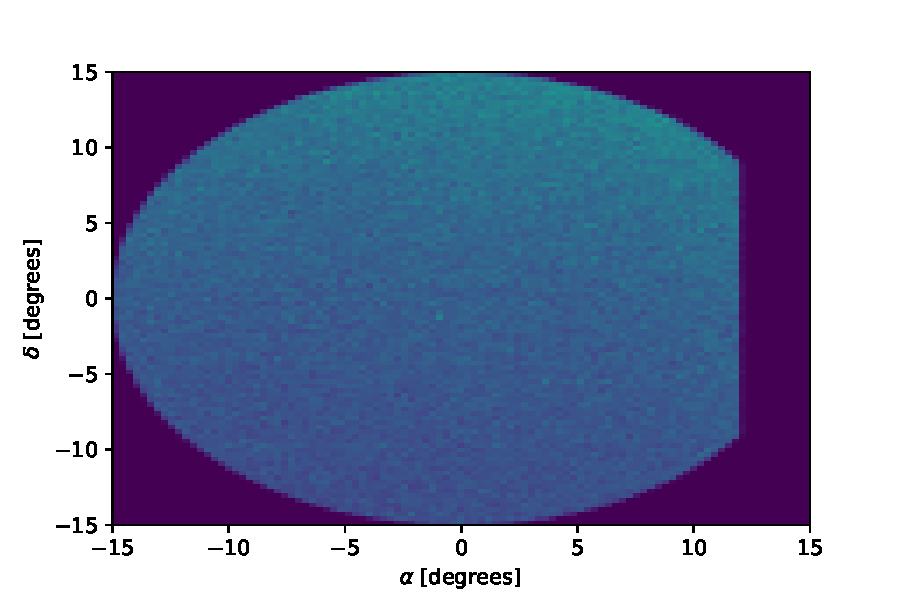
\includegraphics[width=0.5\textwidth]{../figures/histogram2dgaiascan_l101_2_b58_4_ra212_7_dec55_2_npy.pdf}\forloop{imagenum}{0}{\value{imagenum} < 18}{
\includegraphics[width=0.24\textwidth]{../figures/stars_passing_cutgaiascan_l101_2_b58_4_ra212_7_dec55_2_npy_\arabic{imagenum}.pdf}}
\caption{Stars passing cut at Region l$101.2$ b$58.4$ ra$212.7$ dec$55.2$}
\end{figure}

\begin{figure}[h!]
\centering
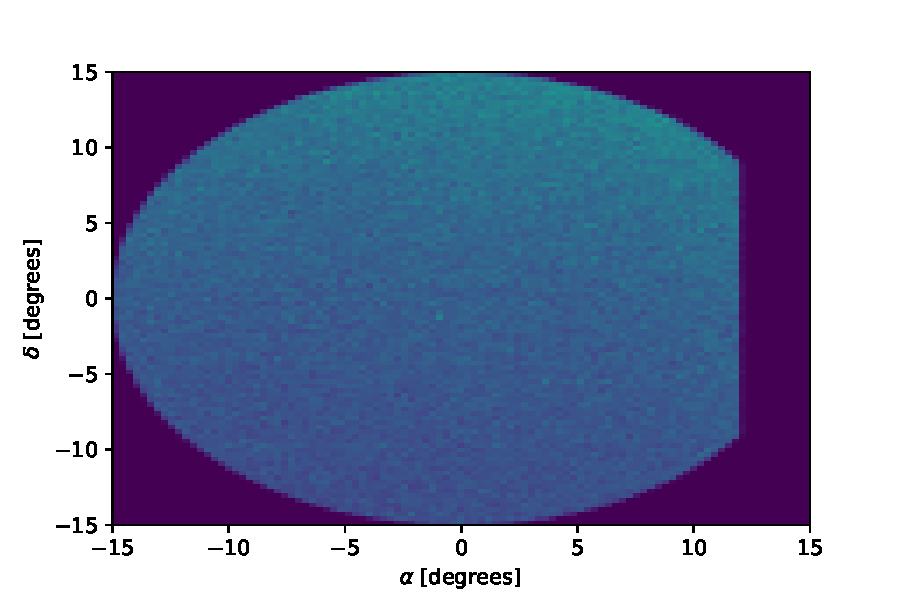
\includegraphics[width=0.5\textwidth]{../figures/histogram2dgaiascan_l101_2_b58_4_ra212_7_dec55_2_npy.pdf}\forloop{imagenum}{0}{\value{imagenum} < 18}{
\includegraphics[width=0.24\textwidth]{../figures/stars_passing_cut_rahistgaiascan_l101_2_b58_4_ra212_7_dec55_2_npy_\arabic{imagenum}.pdf}}
\caption{Stars passing cut at Region l$101.2$ b$58.4$ ra$212.7$ dec$55.2$}
\end{figure}

\begin{figure}[h!]
\centering
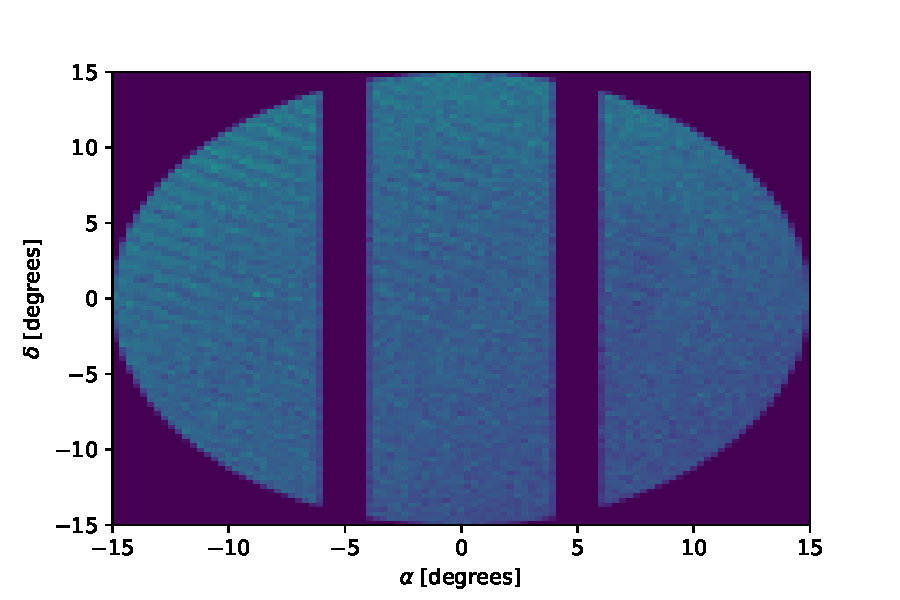
\includegraphics[width=0.5\textwidth]{../figures/histogram2dgaiascan_l22_5_b74_4_ra209_6_dec23_3_npy.pdf}\forloop{imagenum}{0}{\value{imagenum} < 18}{
\includegraphics[width=0.24\textwidth]{../figures/scanning_plotsgaiascan_l22_5_b74_4_ra209_6_dec23_3_npy_\arabic{imagenum}.pdf}}
\caption{Region l$22.5$ b$74.4$ ra$209.6$ dec$23.3$}
\end{figure}

\begin{figure}[h!]
\centering
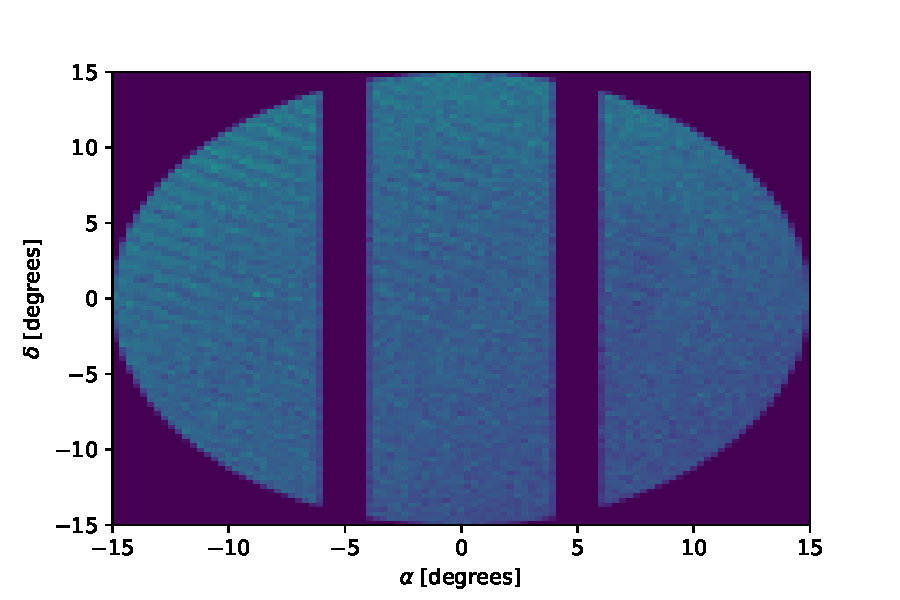
\includegraphics[width=0.5\textwidth]{../figures/histogram2dgaiascan_l22_5_b74_4_ra209_6_dec23_3_npy.pdf}\forloop{imagenum}{0}{\value{imagenum} < 18}{
\includegraphics[width=0.24\textwidth]{../figures/stars_near_zero_2dhistgaiascan_l22_5_b74_4_ra209_6_dec23_3_npy_\arabic{imagenum}.pdf}}
\caption{Region l$22.5$ b$74.4$ ra$209.6$ dec$23.3$}
\end{figure}

\begin{figure}[h!]
\centering
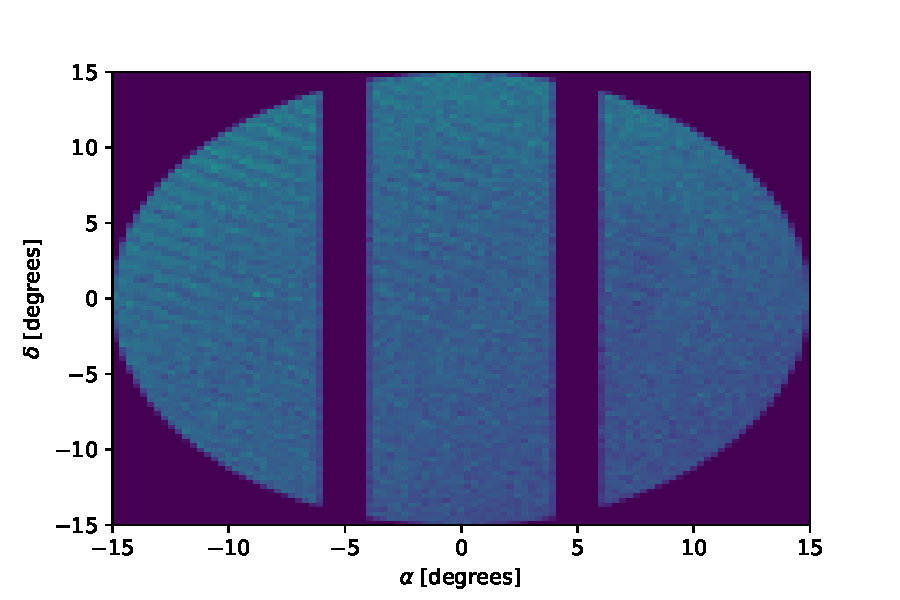
\includegraphics[width=0.5\textwidth]{../figures/histogram2dgaiascan_l22_5_b74_4_ra209_6_dec23_3_npy.pdf}\forloop{imagenum}{0}{\value{imagenum} < 18}{
\includegraphics[width=0.24\textwidth]{../figures/stars_near_zero_rahistgaiascan_l22_5_b74_4_ra209_6_dec23_3_npy_\arabic{imagenum}.pdf}}
\caption{Region l$22.5$ b$74.4$ ra$209.6$ dec$23.3$}
\end{figure}

\begin{figure}[h!]
\centering
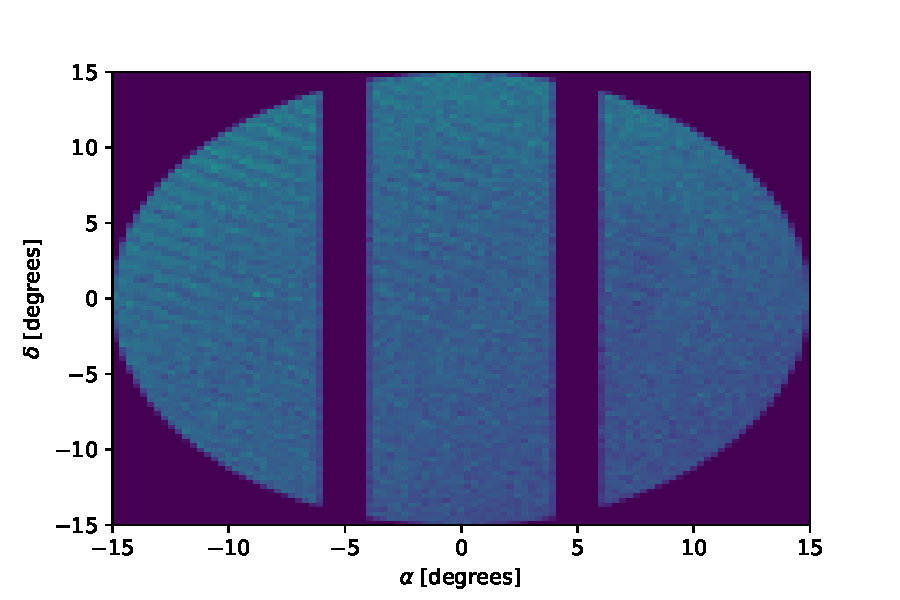
\includegraphics[width=0.5\textwidth]{../figures/histogram2dgaiascan_l22_5_b74_4_ra209_6_dec23_3_npy.pdf}\forloop{imagenum}{0}{\value{imagenum} < 18}{
\includegraphics[width=0.24\textwidth]{../figures/stars_passing_cutgaiascan_l22_5_b74_4_ra209_6_dec23_3_npy_\arabic{imagenum}.pdf}}
\caption{Region l$22.5$ b$74.4$ ra$209.6$ dec$23.3$}
\end{figure}

\begin{figure}[h!]
\centering
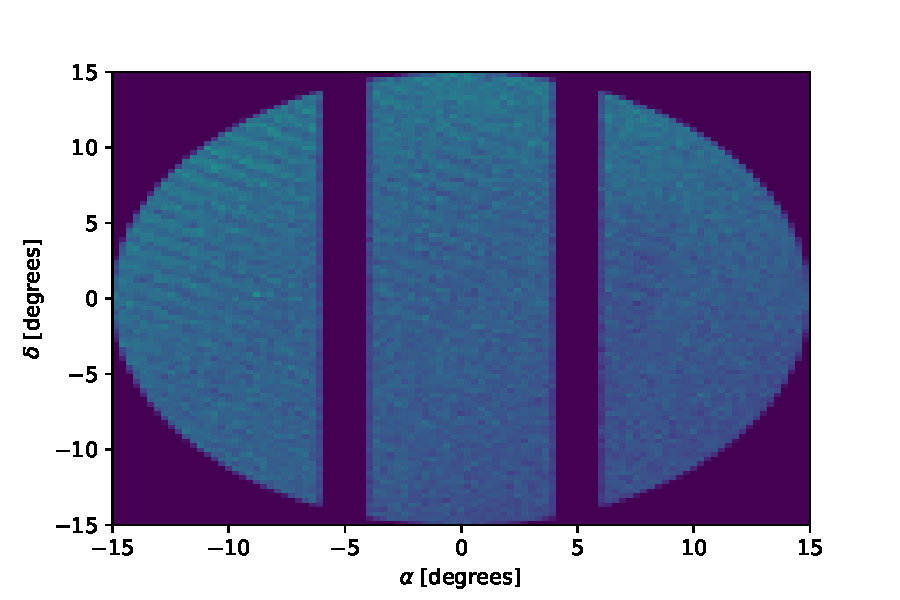
\includegraphics[width=0.5\textwidth]{../figures/histogram2dgaiascan_l22_5_b74_4_ra209_6_dec23_3_npy.pdf}\forloop{imagenum}{0}{\value{imagenum} < 18}{
\includegraphics[width=0.24\textwidth]{../figures/stars_near_zero_rahistgaiascan_l22_5_b74_4_ra209_6_dec23_3_npy_\arabic{imagenum}.pdf}}
\caption{Region l$22.5$ b$74.4$ ra$209.6$ dec$23.3$}
\end{figure}

\begin{figure}[h!]
\centering
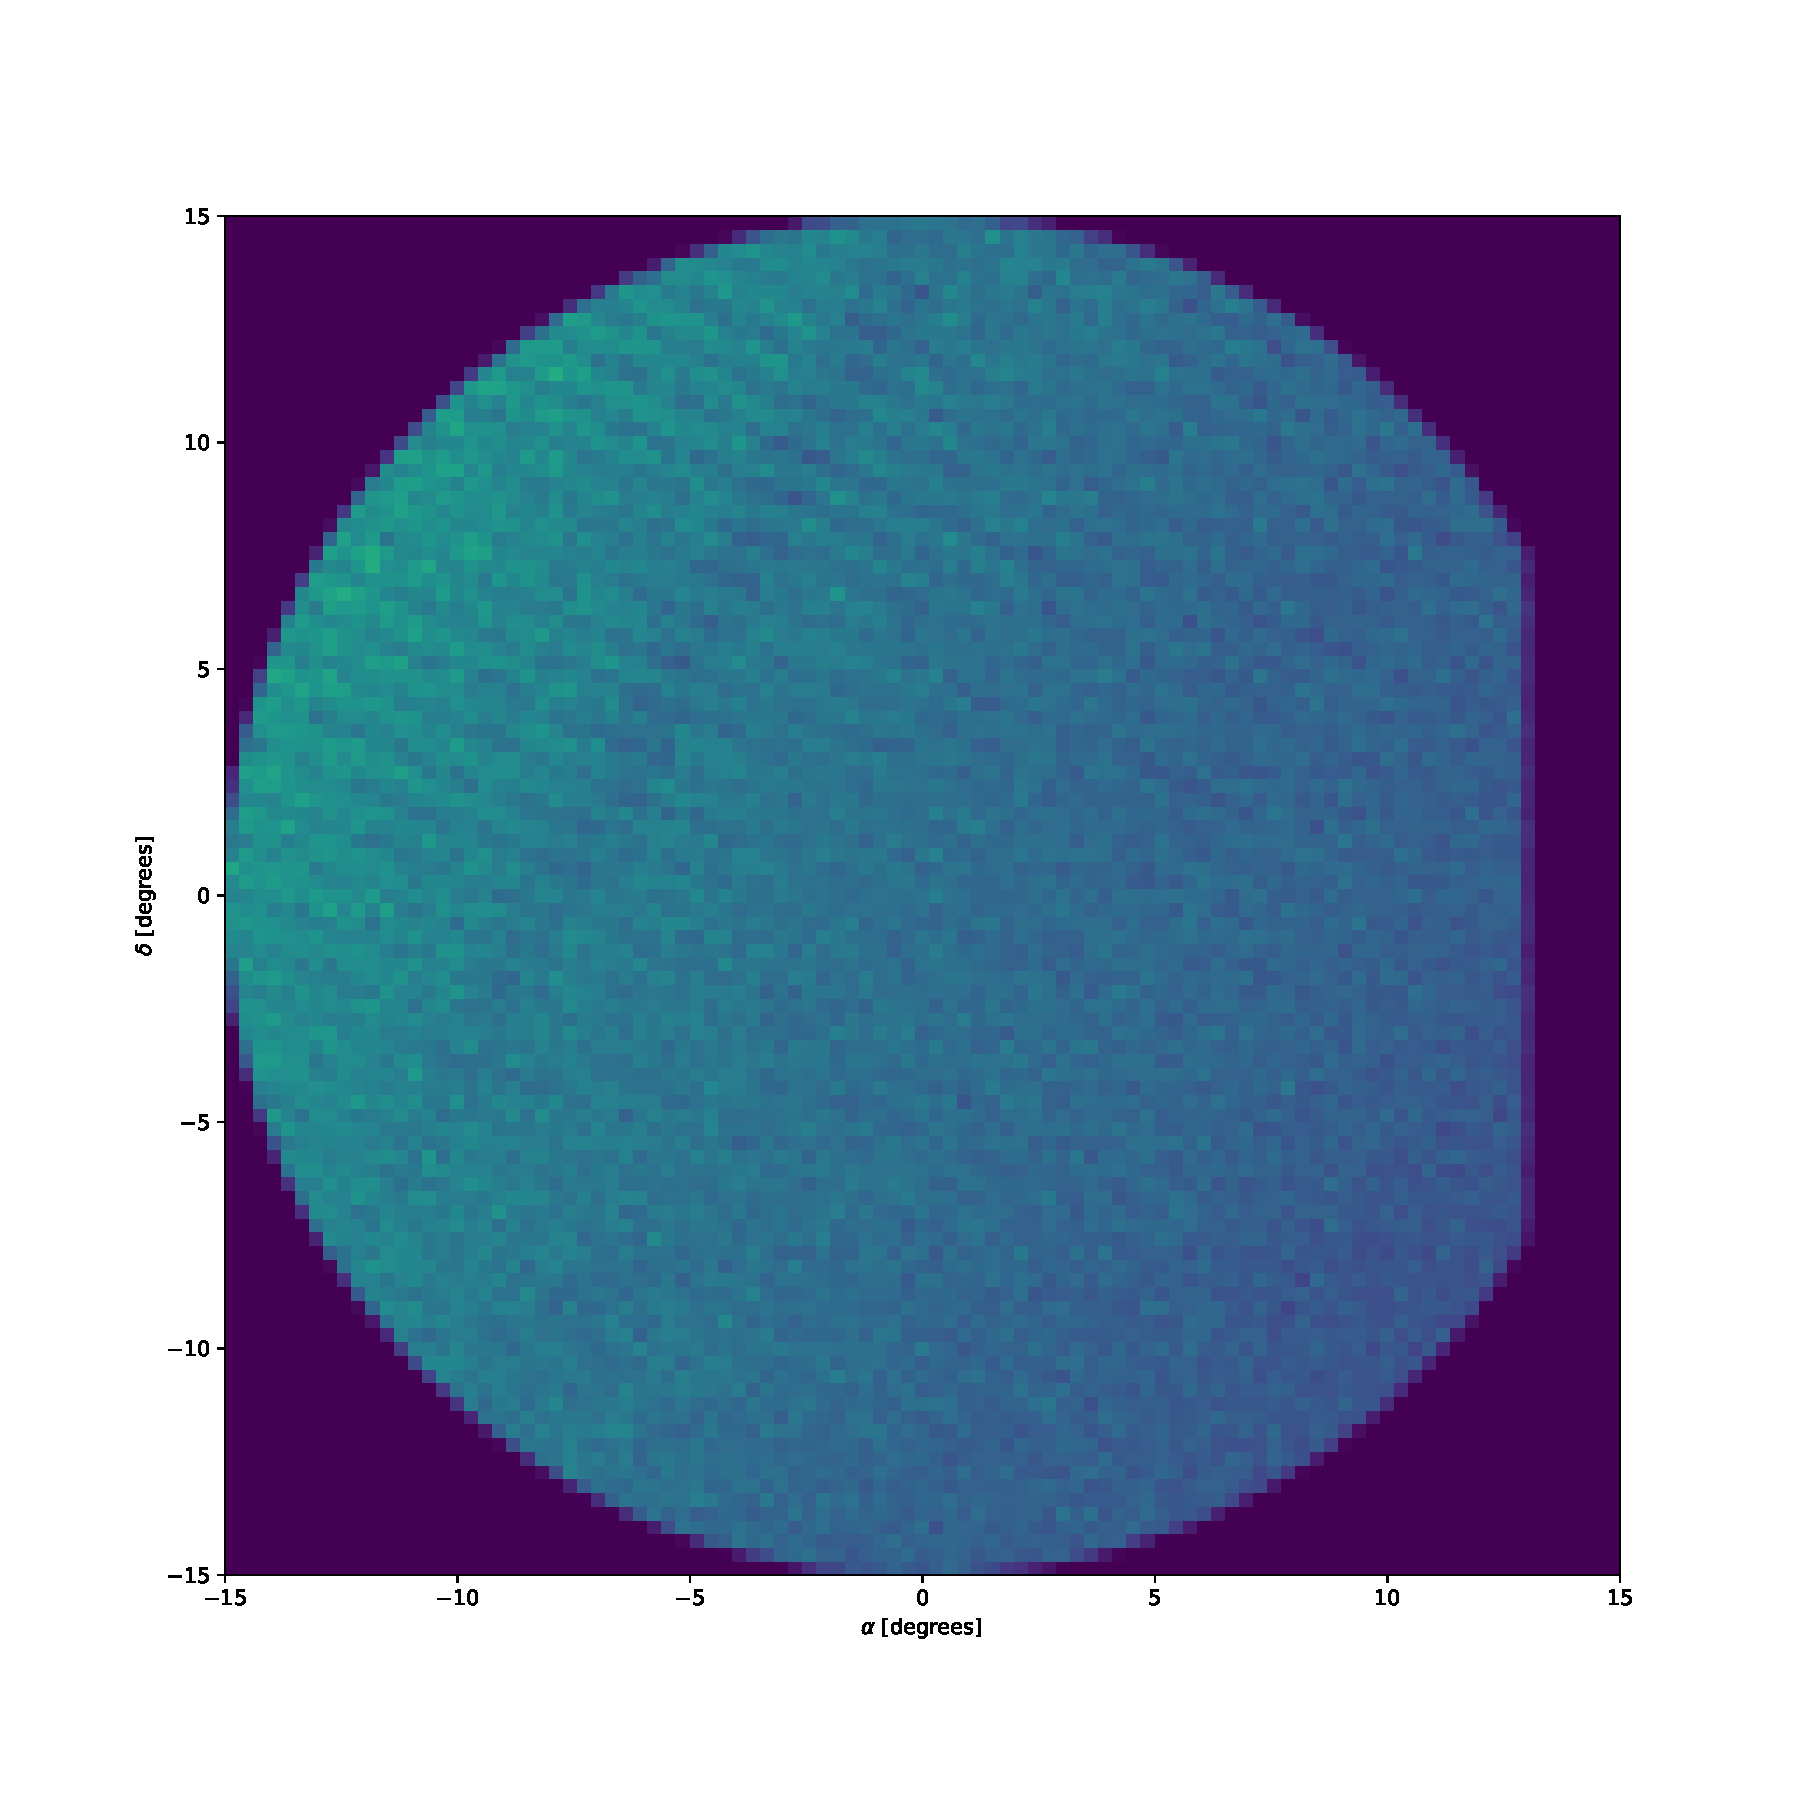
\includegraphics[width=0.5\textwidth]{../figures/histogram2dgaiascan_l315_0_b66_4_ra197_7_dec4_0_npy.pdf}\forloop{imagenum}{0}{\value{imagenum} < 18}{
\includegraphics[width=0.24\textwidth]{../figures/scanning_plotsgaiascan_l315_0_b66_4_ra197_7_dec4_0_npy_\arabic{imagenum}.pdf}}
\caption{Region l$315.0$ b$66.4$ ra$197.7$ dec$4.0$}
\end{figure}

\begin{figure}[h!]
\centering
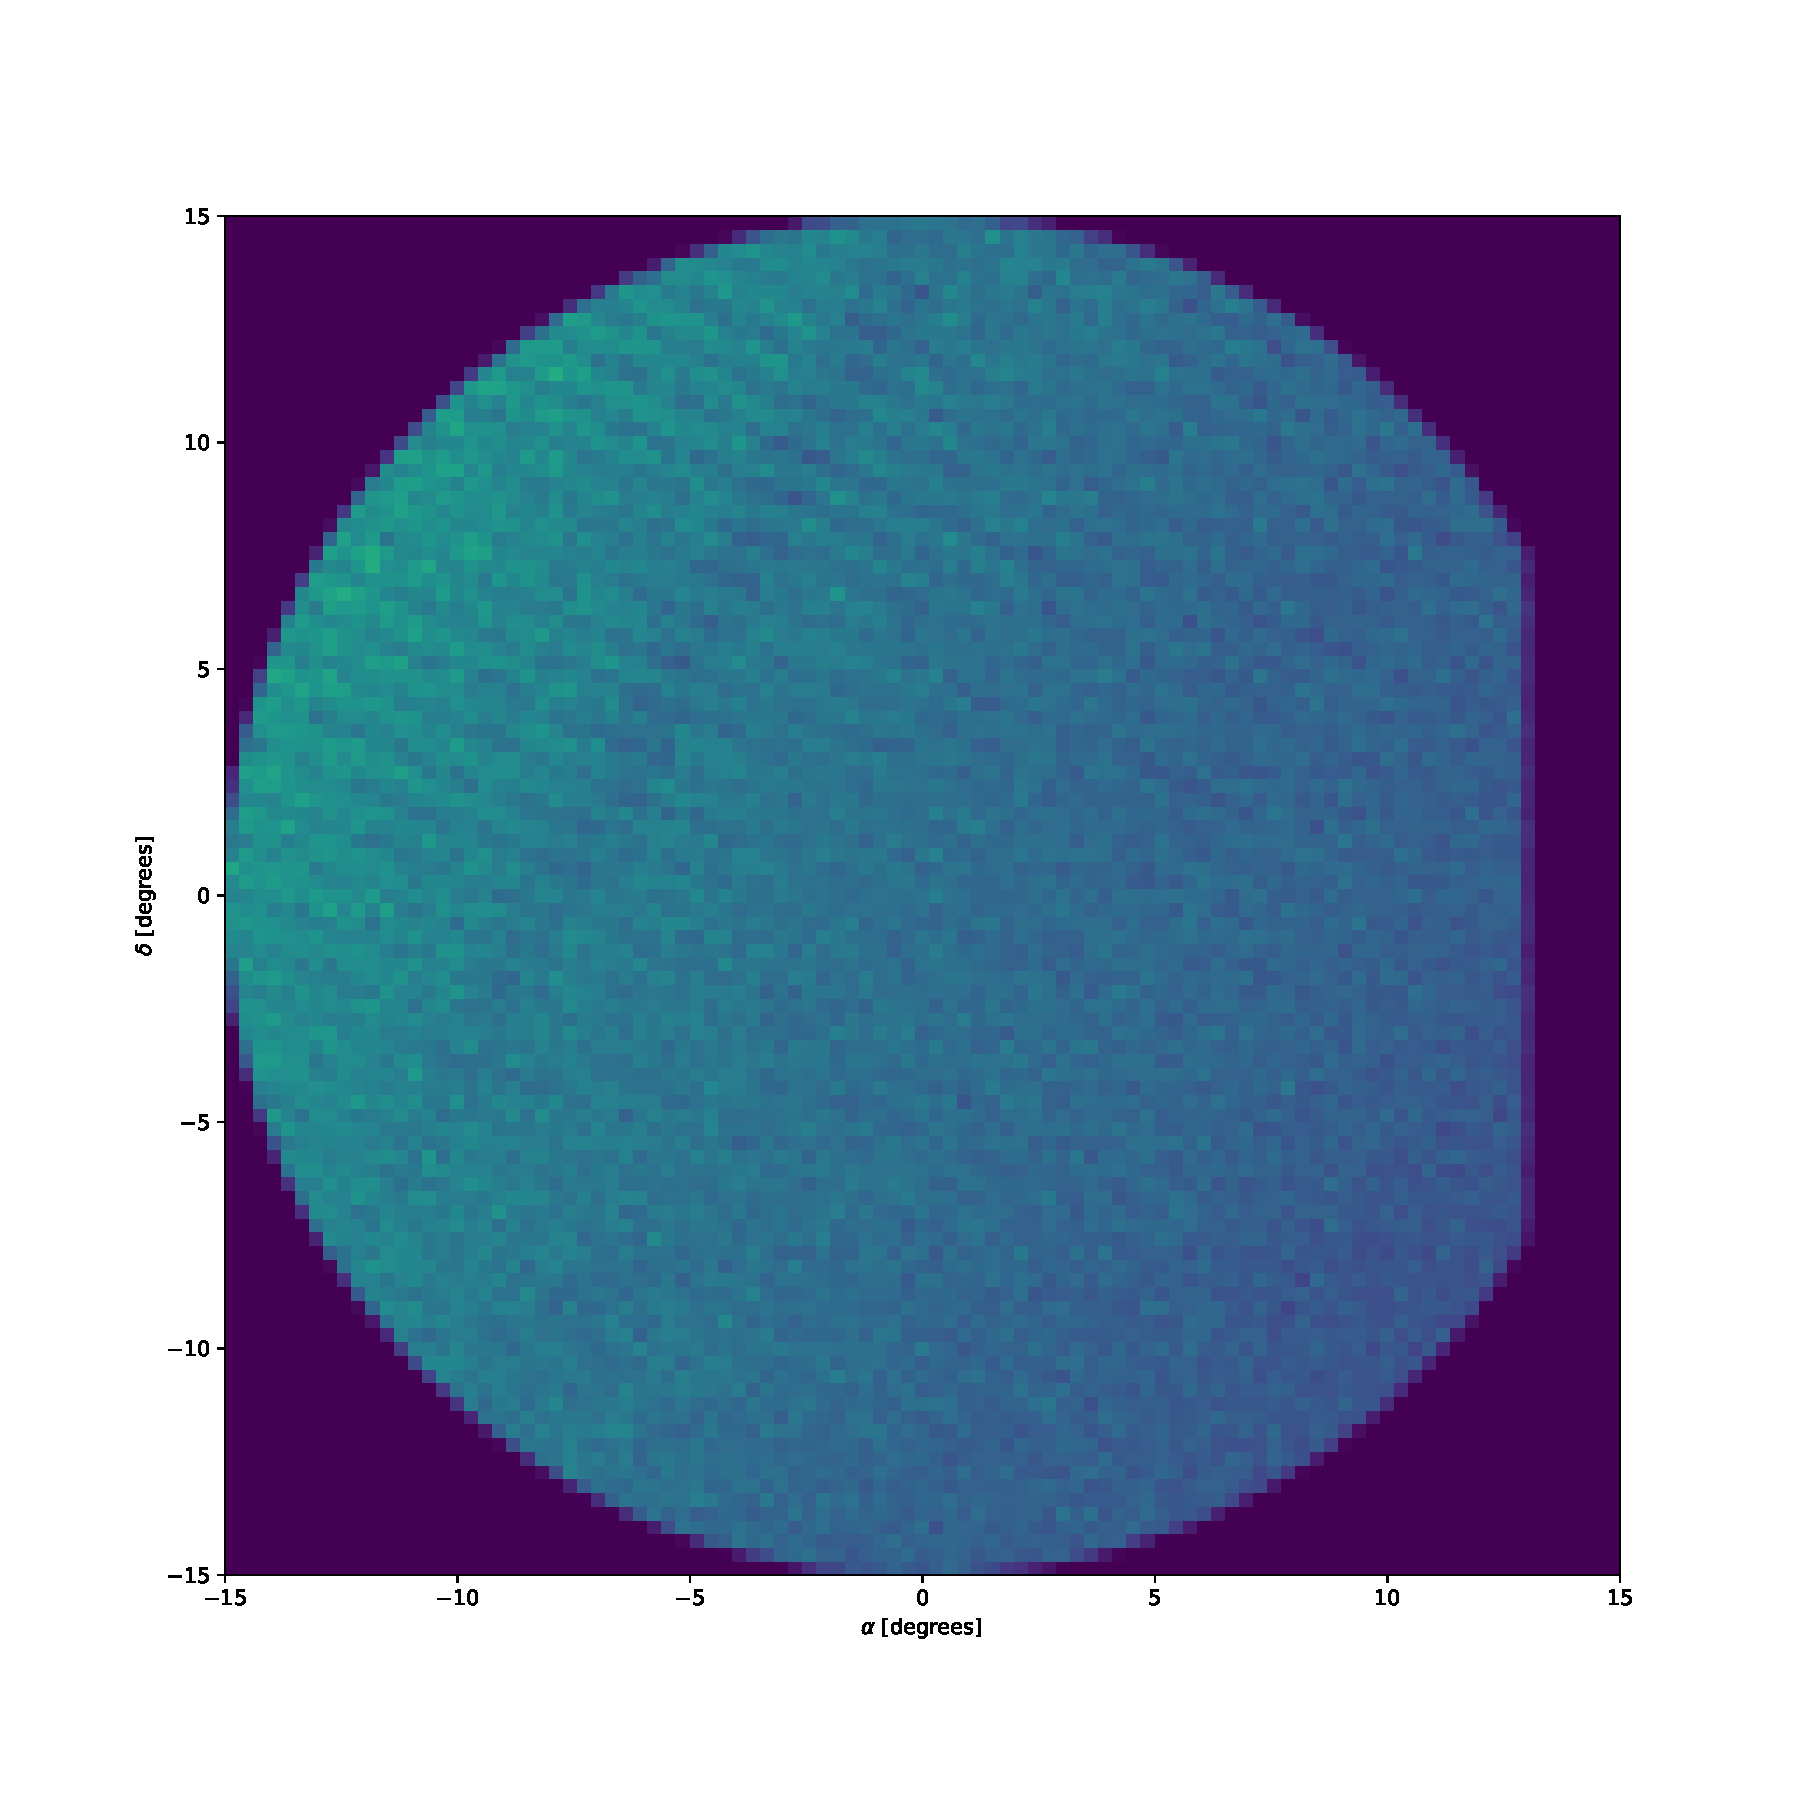
\includegraphics[width=0.5\textwidth]{../figures/histogram2dgaiascan_l315_0_b66_4_ra197_7_dec4_0_npy.pdf}\forloop{imagenum}{0}{\value{imagenum} < 18}{
\includegraphics[width=0.24\textwidth]{../figures/stars_near_zero_2dhistgaiascan_l315_0_b66_4_ra197_7_dec4_0_npy_\arabic{imagenum}.pdf}}
\caption{Region l$315.0$ b$66.4$ ra$197.7$ dec$4.0$}
\end{figure}

\begin{figure}[h!]
\centering
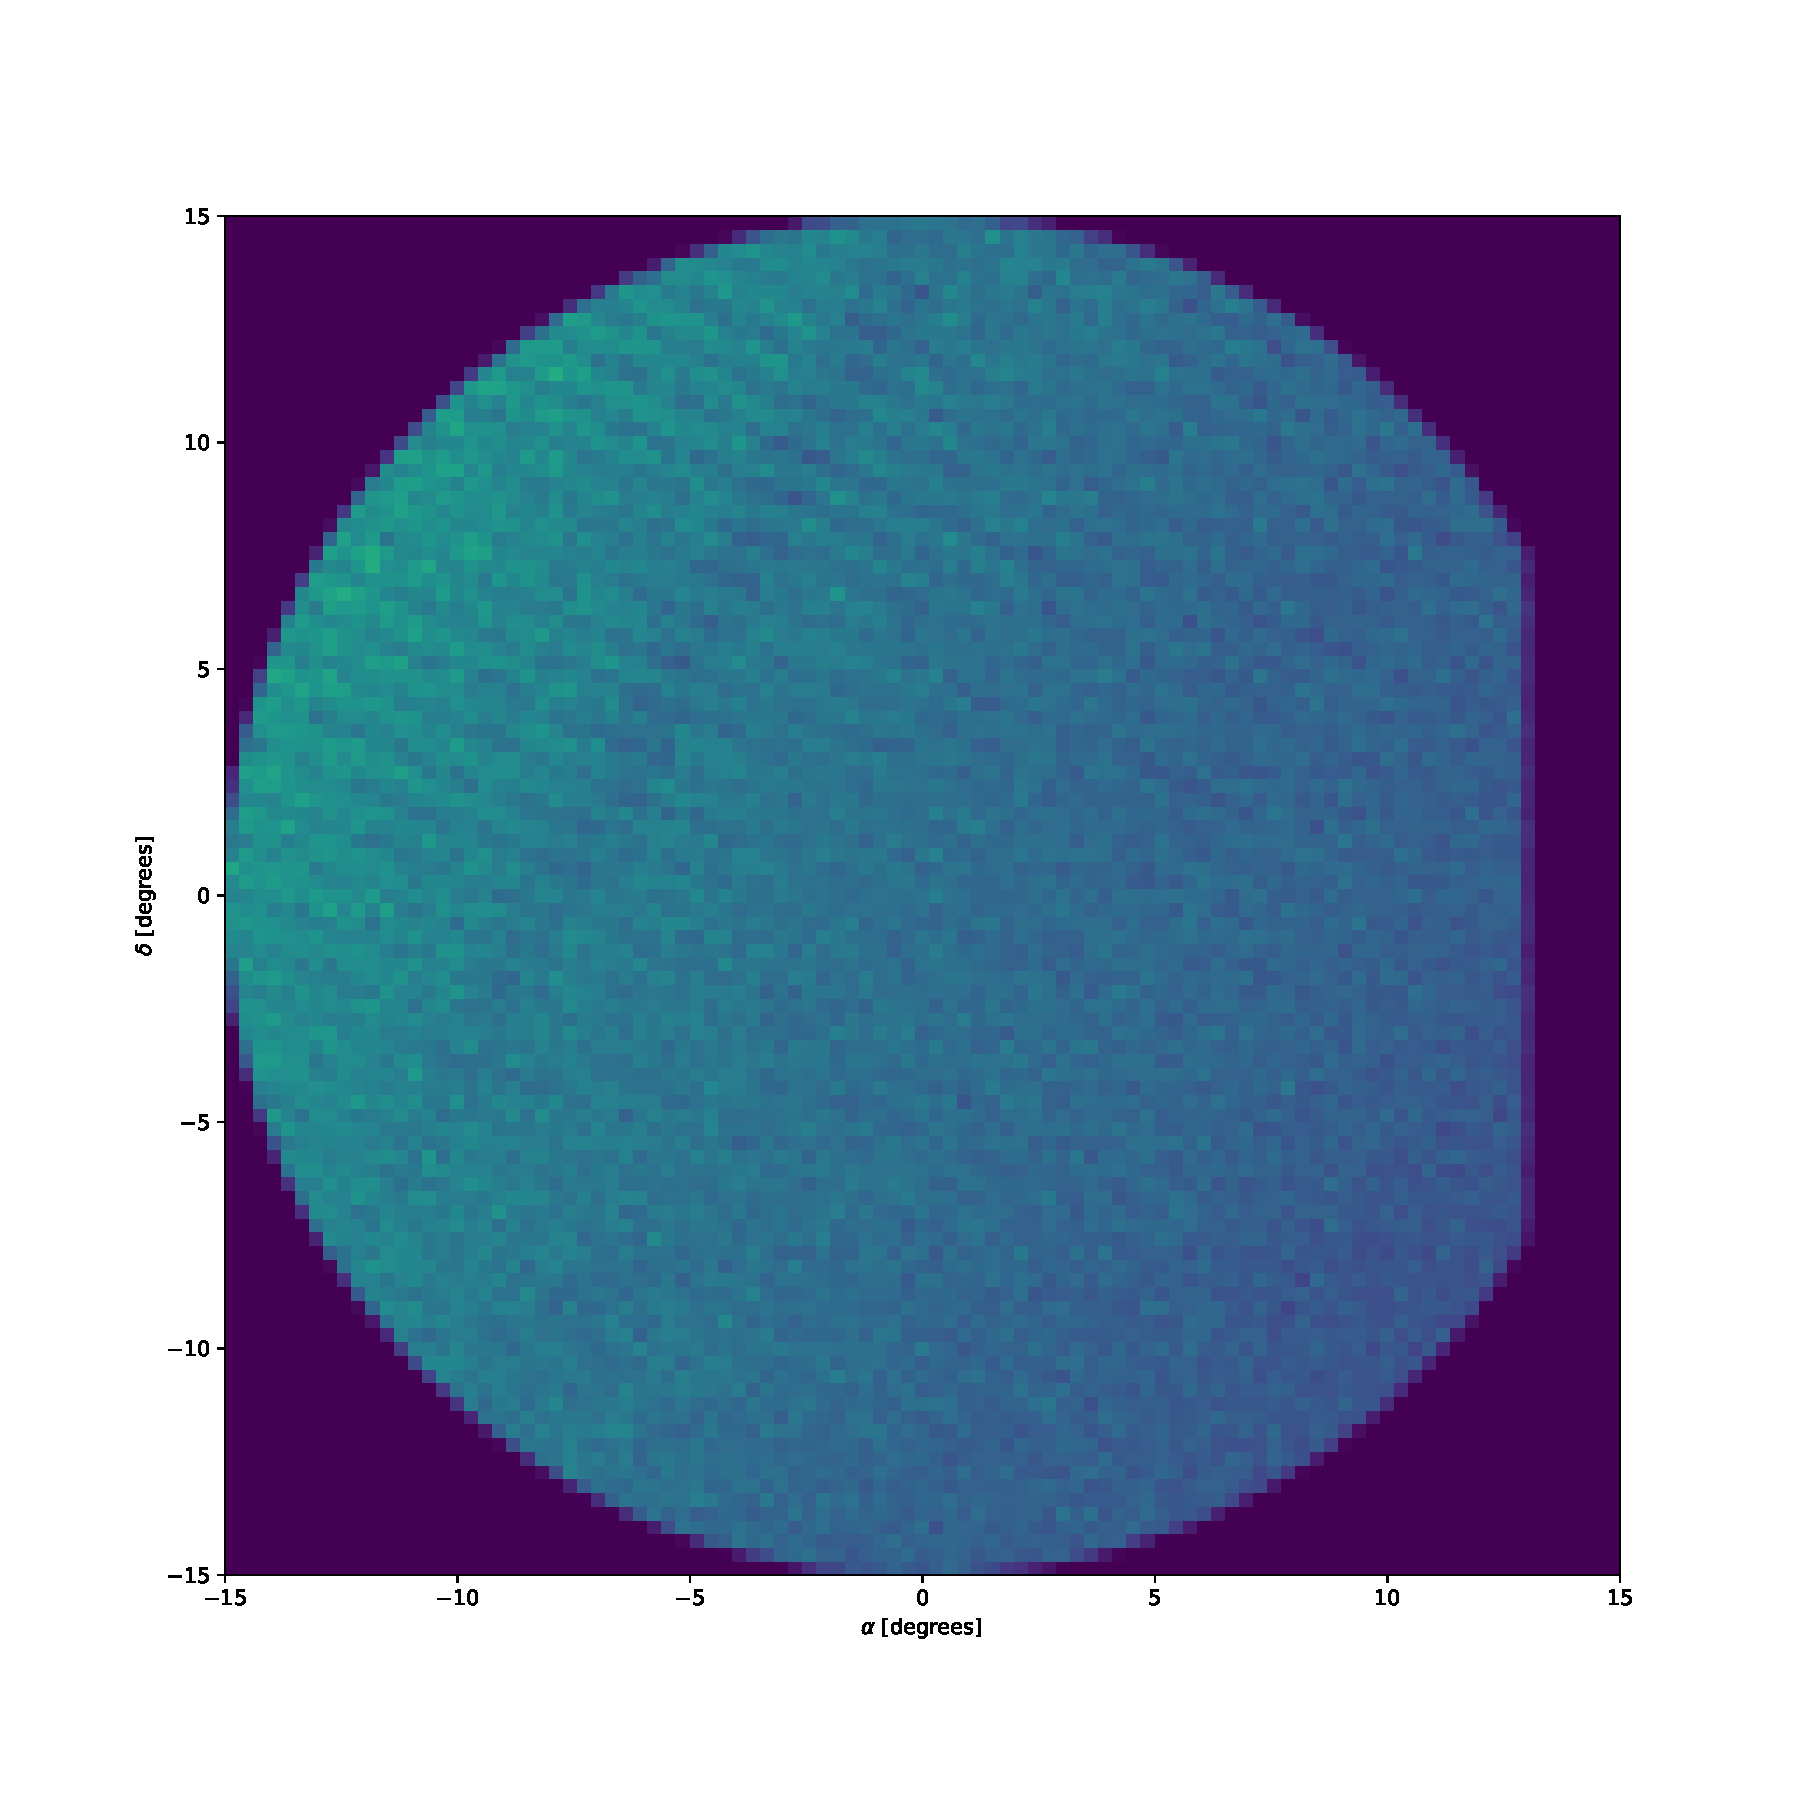
\includegraphics[width=0.5\textwidth]{../figures/histogram2dgaiascan_l315_0_b66_4_ra197_7_dec4_0_npy.pdf}\forloop{imagenum}{0}{\value{imagenum} < 18}{
\includegraphics[width=0.24\textwidth]{../figures/stars_near_zero_rahistgaiascan_l315_0_b66_4_ra197_7_dec4_0_npy_\arabic{imagenum}.pdf}}
\caption{Region l$315.0$ b$66.4$ ra$197.7$ dec$4.0$}
\end{figure}

\begin{figure}[h!]
\centering
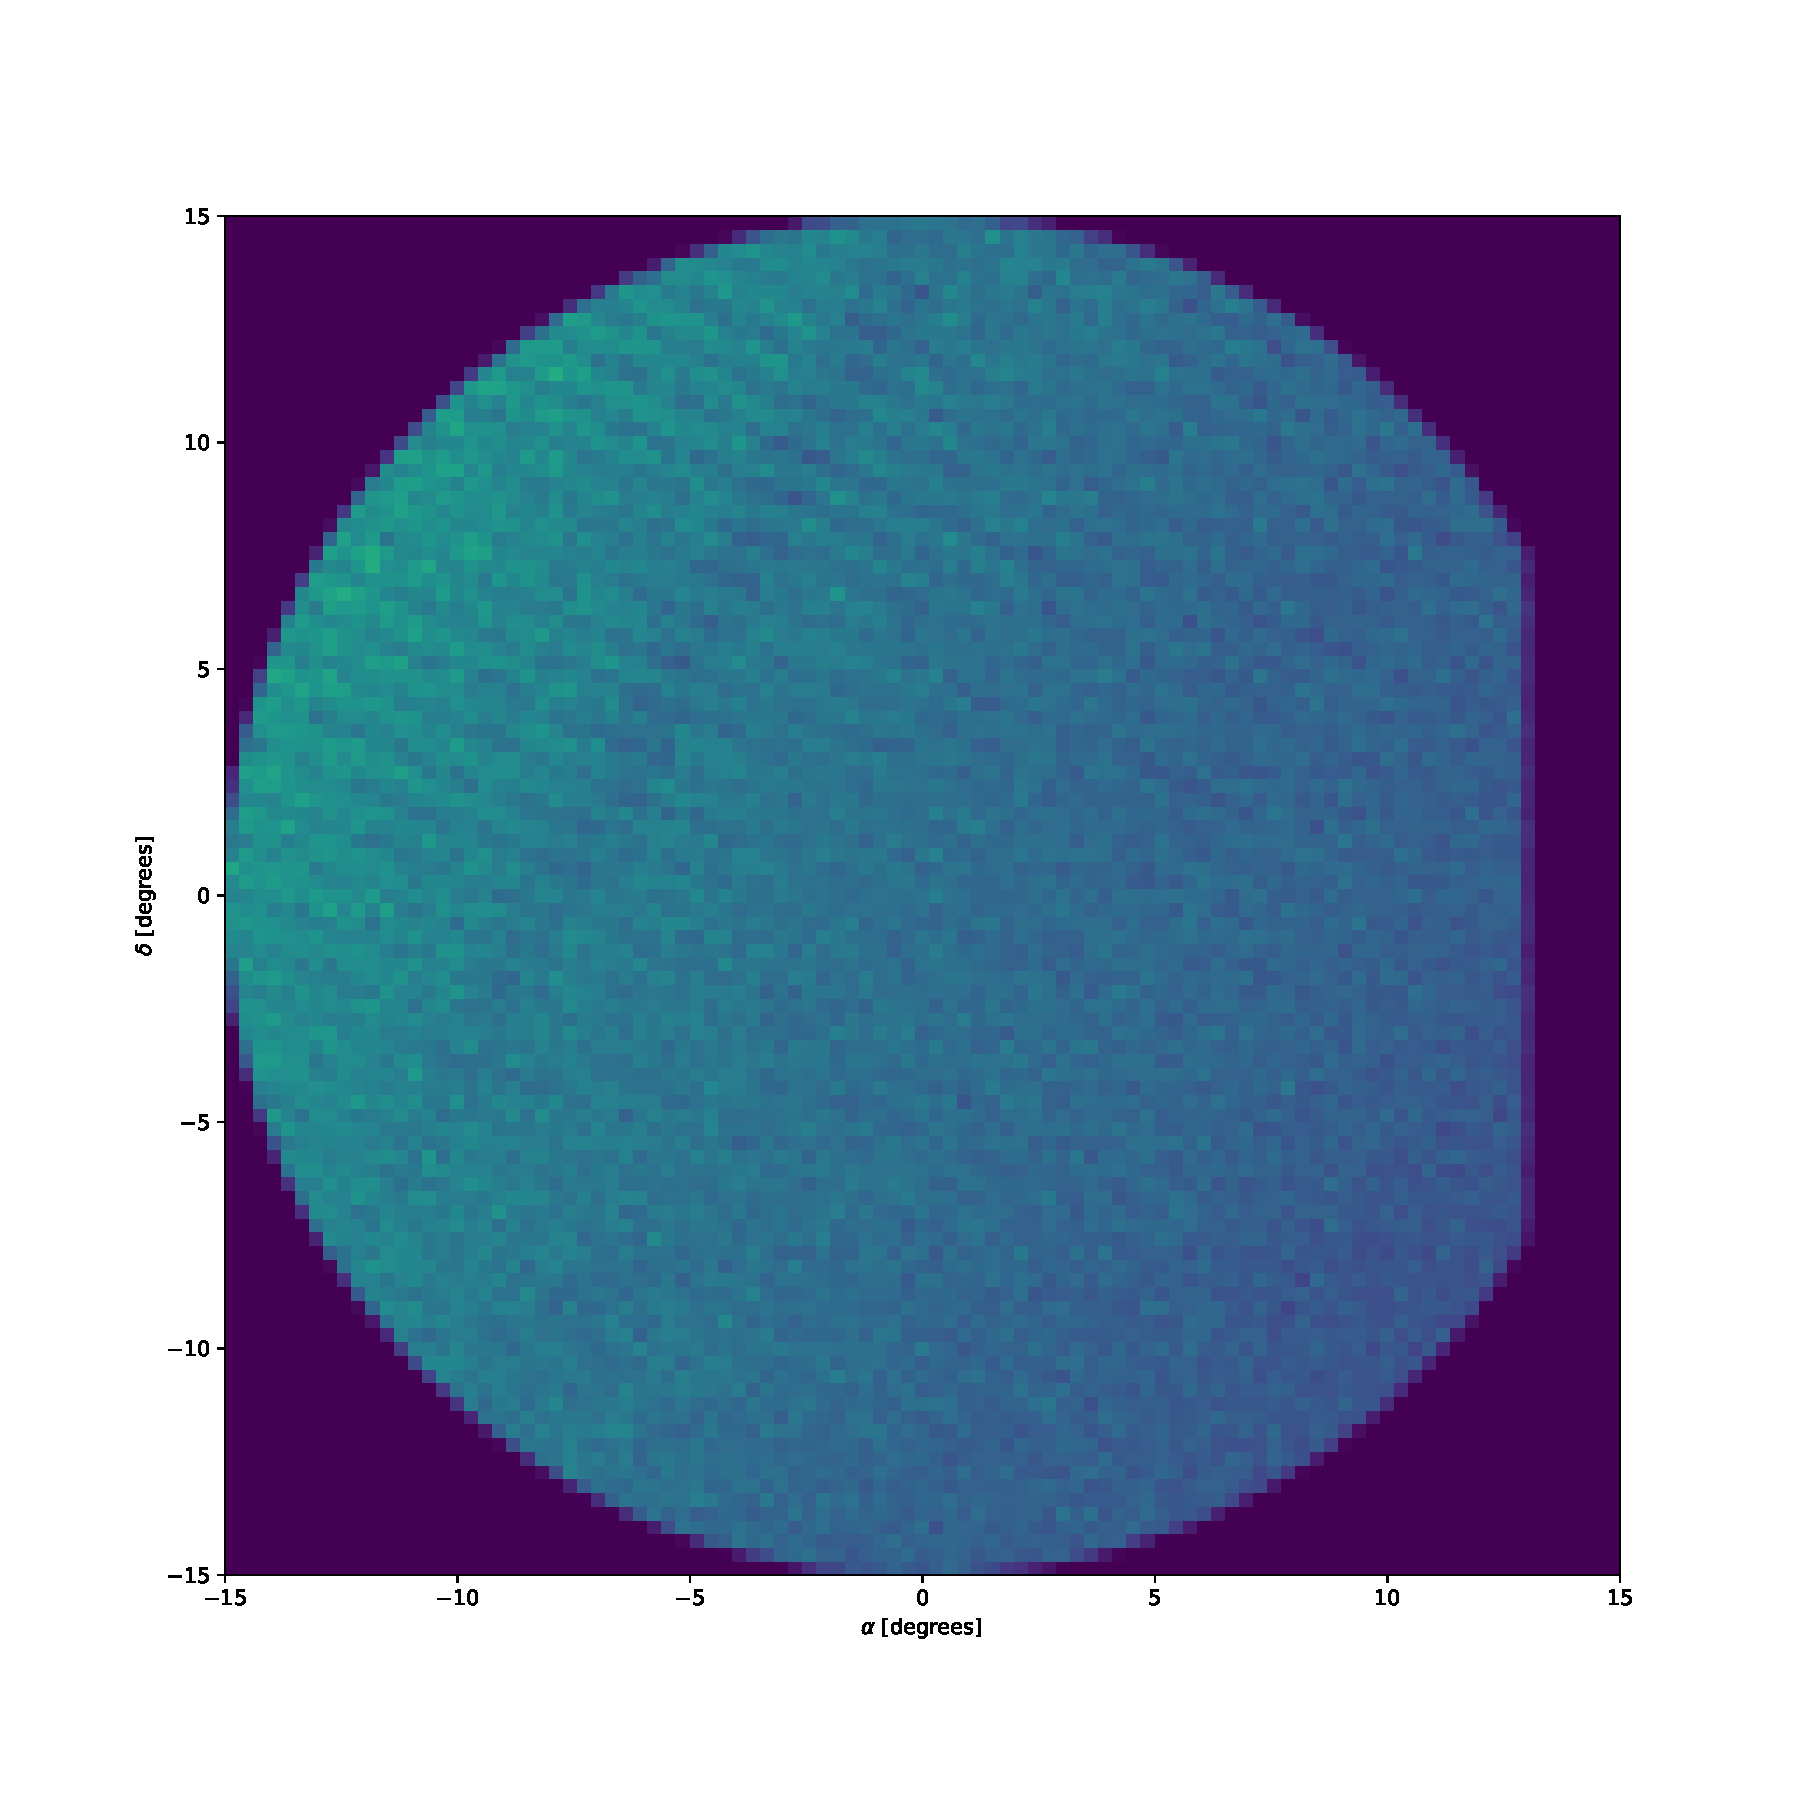
\includegraphics[width=0.5\textwidth]{../figures/histogram2dgaiascan_l315_0_b66_4_ra197_7_dec4_0_npy.pdf}\forloop{imagenum}{0}{\value{imagenum} < 18}{
\includegraphics[width=0.24\textwidth]{../figures/stars_passing_cutgaiascan_l315_0_b66_4_ra197_7_dec4_0_npy_\arabic{imagenum}.pdf}}
\caption{Region l$315.0$ b$66.4$ ra$197.7$ dec$4.0$}
\end{figure}

\begin{figure}[h!]
\centering
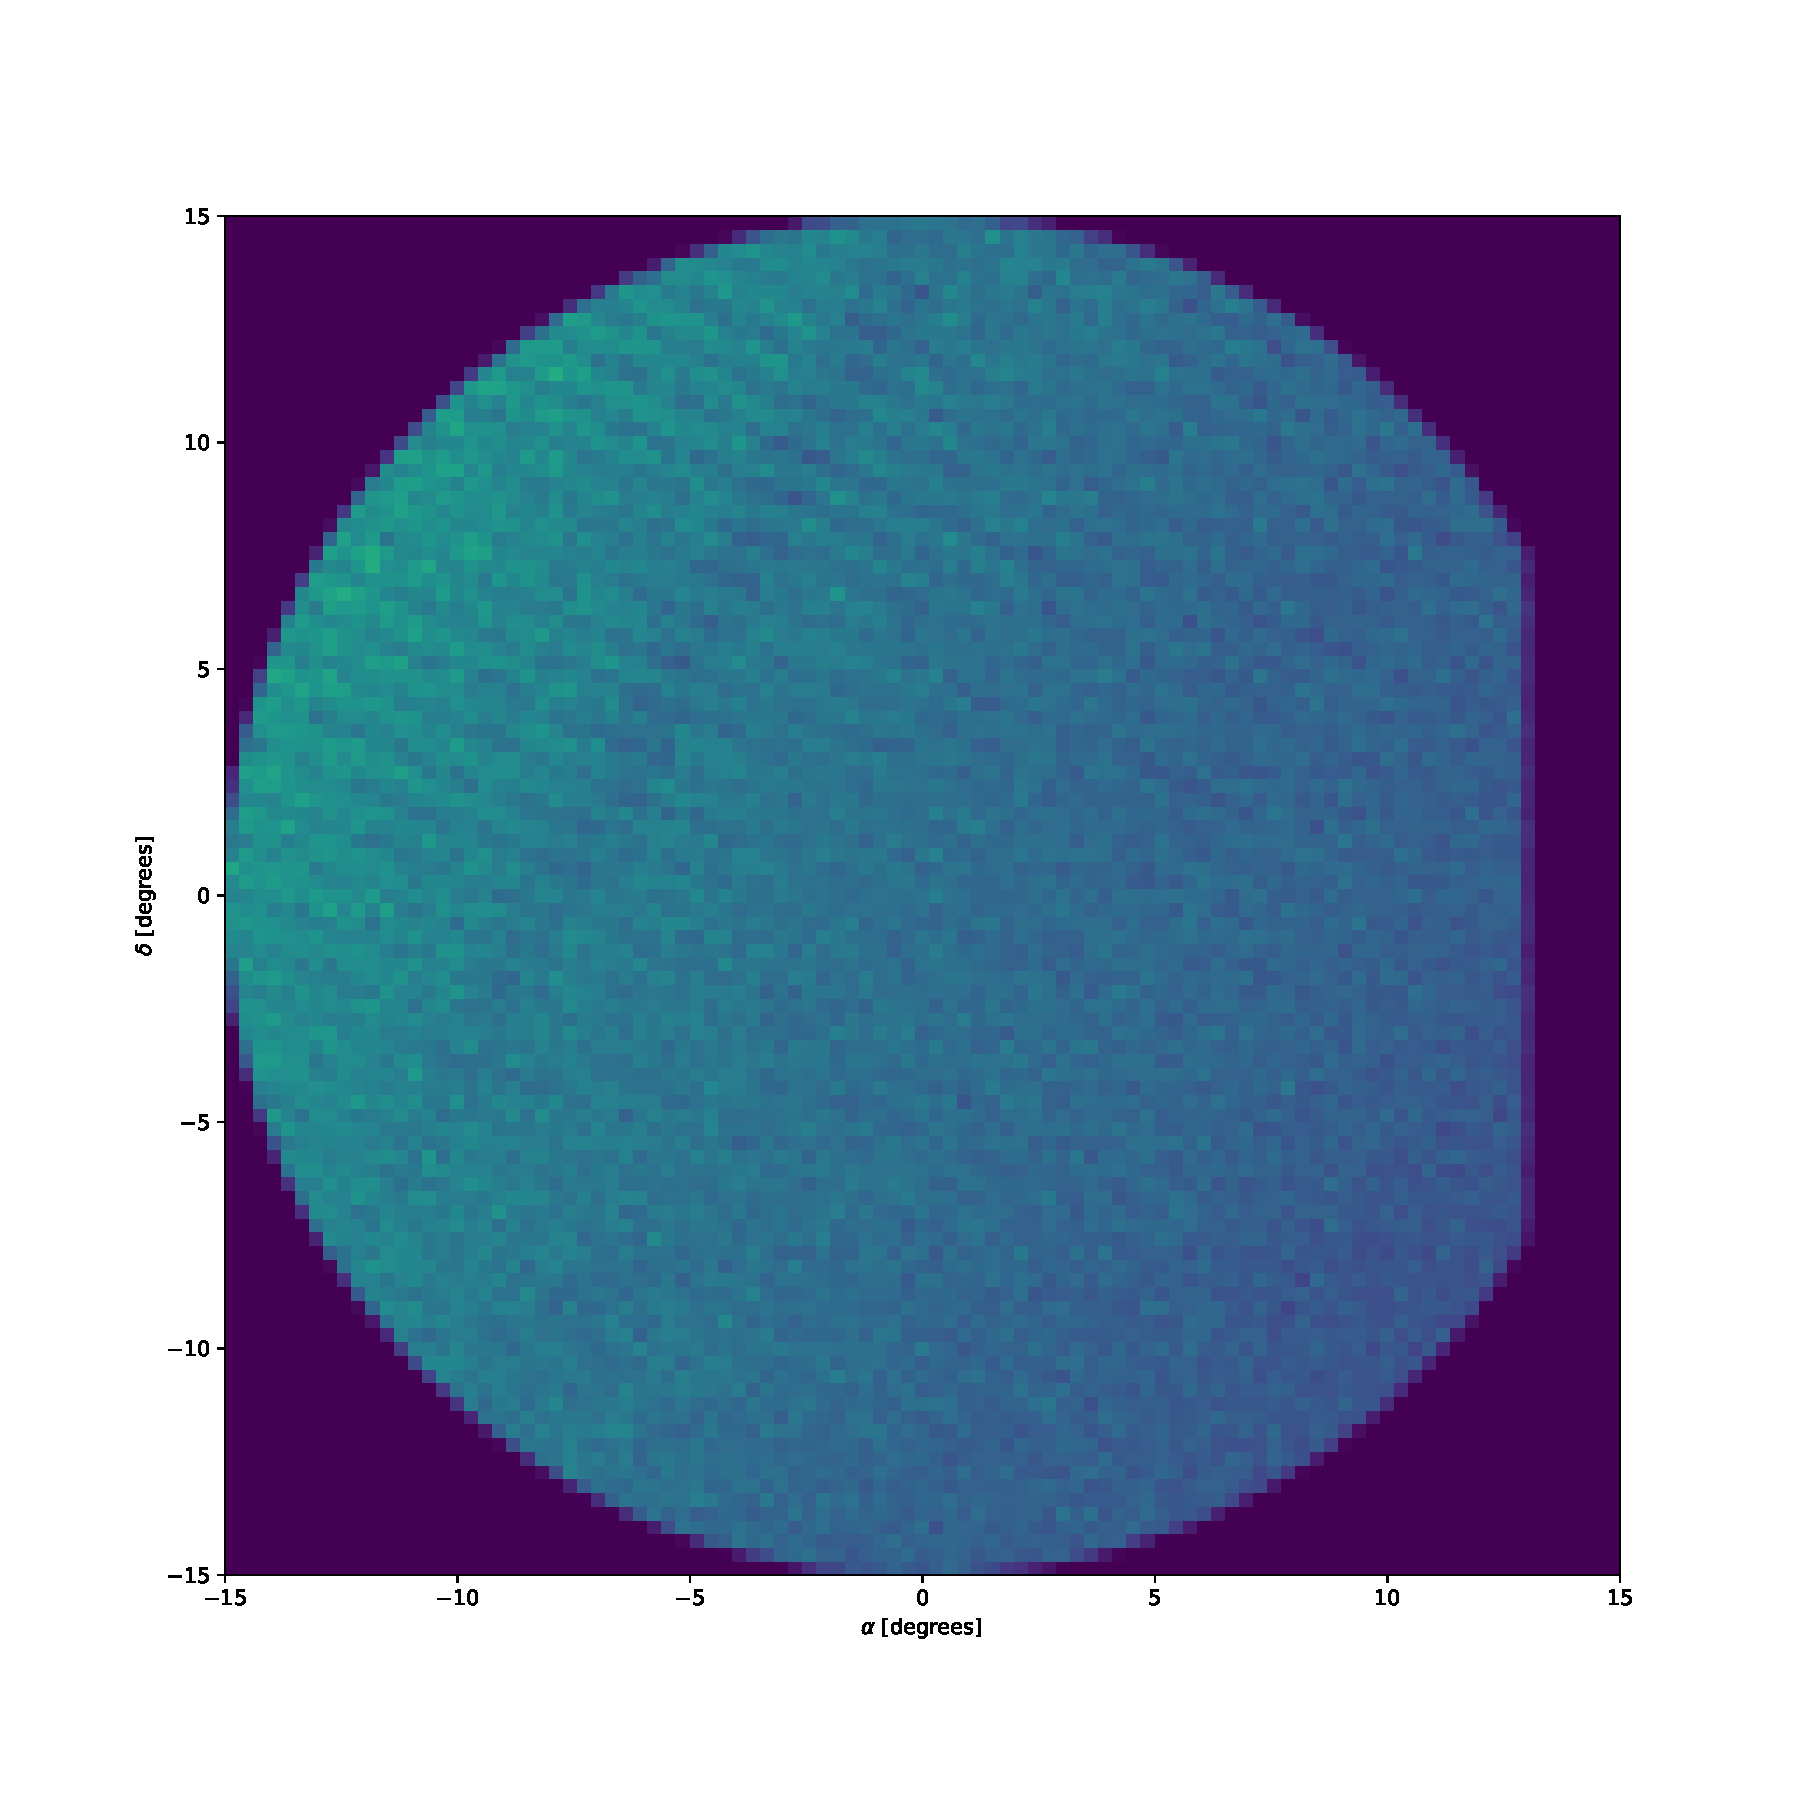
\includegraphics[width=0.5\textwidth]{../figures/histogram2dgaiascan_l315_0_b66_4_ra197_7_dec4_0_npy.pdf}\forloop{imagenum}{0}{\value{imagenum} < 18}{
\includegraphics[width=0.24\textwidth]{../figures/stars_passing_cut_rahistgaiascan_l315_0_b66_4_ra197_7_dec4_0_npy_\arabic{imagenum}.pdf}}
\caption{Region l$315.0$ b$66.4$ ra$197.7$ dec$4.0$}
\end{figure}

\begin{figure}[h!]
\centering
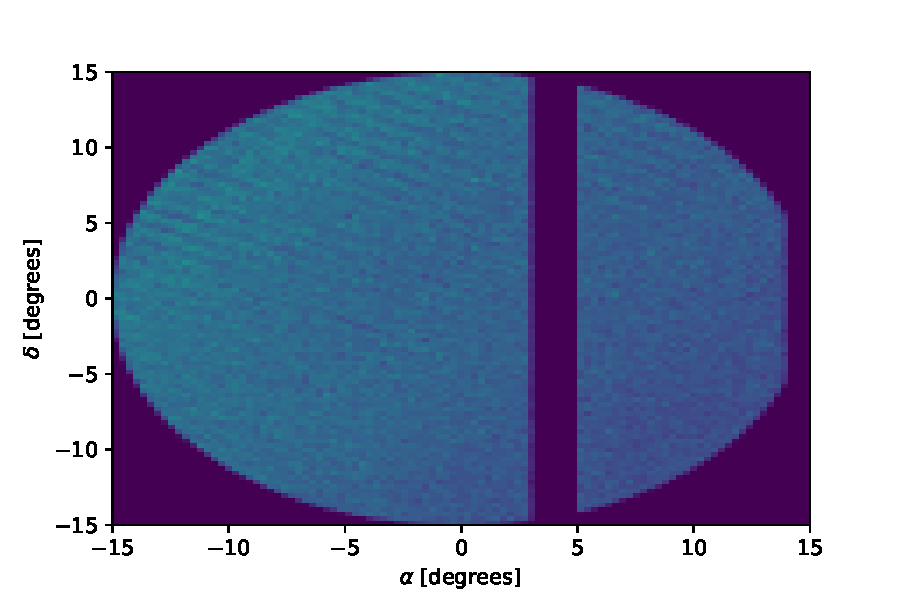
\includegraphics[width=0.5\textwidth]{../figures/histogram2dgaiascan_l337_5_b74_4_ra201_9_dec14_0_npy.pdf}\forloop{imagenum}{0}{\value{imagenum} < 18}{
\includegraphics[width=0.24\textwidth]{../figures/scanning_plotsgaiascan_l337_5_b74_4_ra201_9_dec14_0_npy_\arabic{imagenum}.pdf}}
\caption{Region l$337.5$ b$74.4$ ra$201.9$ dec$14.0$}
\end{figure}

\begin{figure}[h!]
\centering
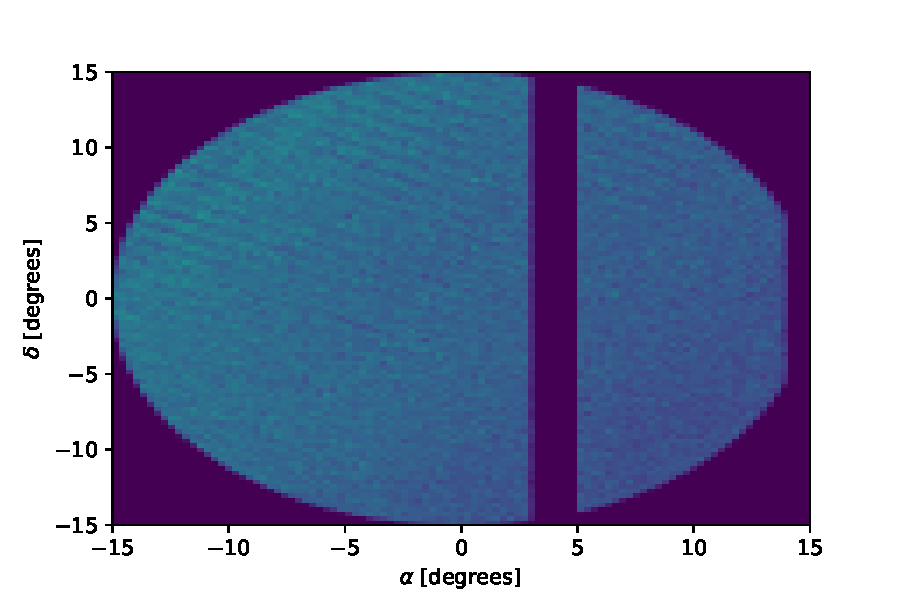
\includegraphics[width=0.5\textwidth]{../figures/histogram2dgaiascan_l337_5_b74_4_ra201_9_dec14_0_npy.pdf}\forloop{imagenum}{0}{\value{imagenum} < 18}{
\includegraphics[width=0.24\textwidth]{../figures/stars_near_zero_2dhistgaiascan_l337_5_b74_4_ra201_9_dec14_0_npy_\arabic{imagenum}.pdf}}
\caption{Region l$337.5$ b$74.4$ ra$201.9$ dec$14.0$}
\end{figure}

\begin{figure}[h!]
\centering
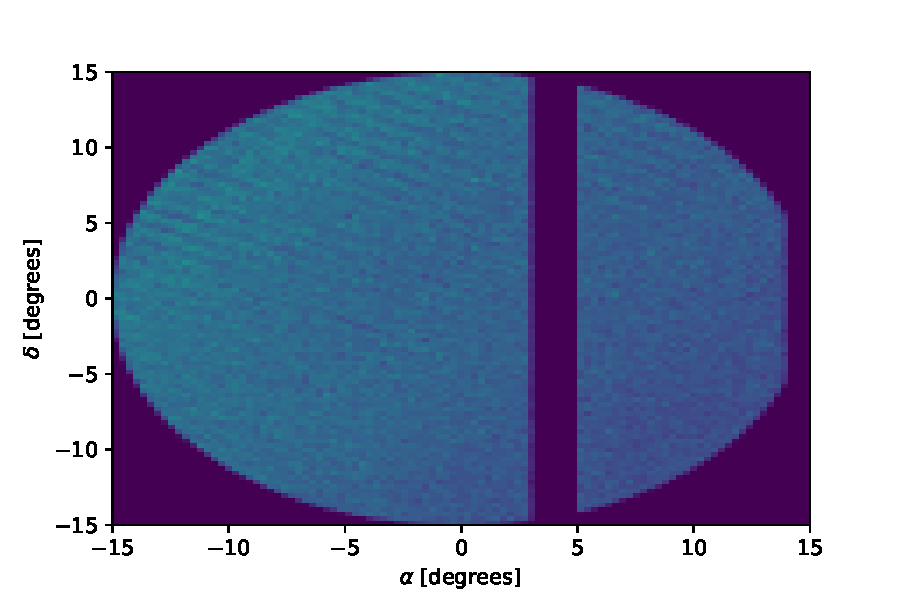
\includegraphics[width=0.5\textwidth]{../figures/histogram2dgaiascan_l337_5_b74_4_ra201_9_dec14_0_npy.pdf}\forloop{imagenum}{0}{\value{imagenum} < 18}{
\includegraphics[width=0.24\textwidth]{../figures/stars_near_zero_rahistgaiascan_l337_5_b74_4_ra201_9_dec14_0_npy_\arabic{imagenum}.pdf}}
\caption{Region l$337.5$ b$74.4$ ra$201.9$ dec$14.0$}
\end{figure}

\begin{figure}[h!]
\centering
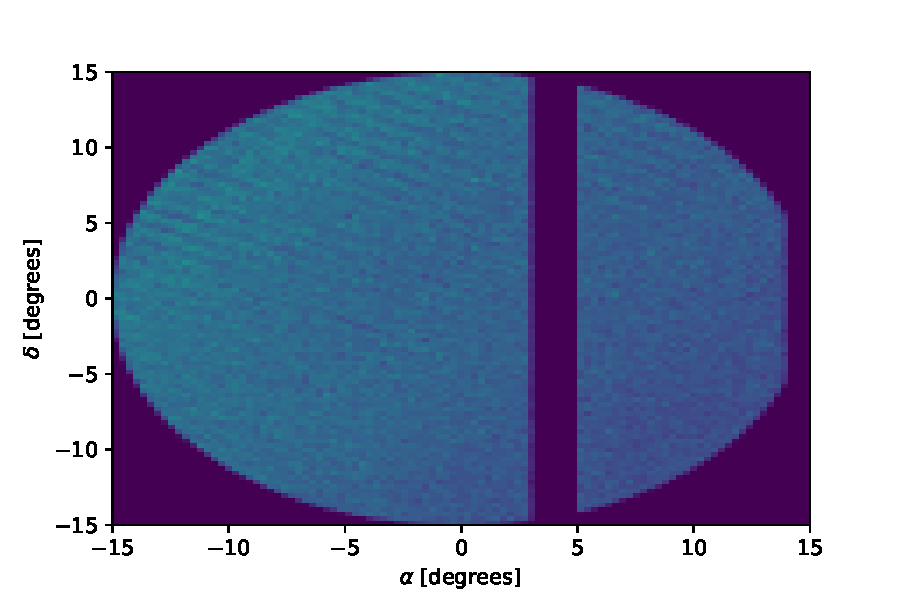
\includegraphics[width=0.5\textwidth]{../figures/histogram2dgaiascan_l337_5_b74_4_ra201_9_dec14_0_npy.pdf}\forloop{imagenum}{0}{\value{imagenum} < 18}{
\includegraphics[width=0.24\textwidth]{../figures/stars_passing_cutgaiascan_l337_5_b74_4_ra201_9_dec14_0_npy_\arabic{imagenum}.pdf}}
\caption{Region l$337.5$ b$74.4$ ra$201.9$ dec$14.0$}
\end{figure}

\begin{figure}[h!]
\centering
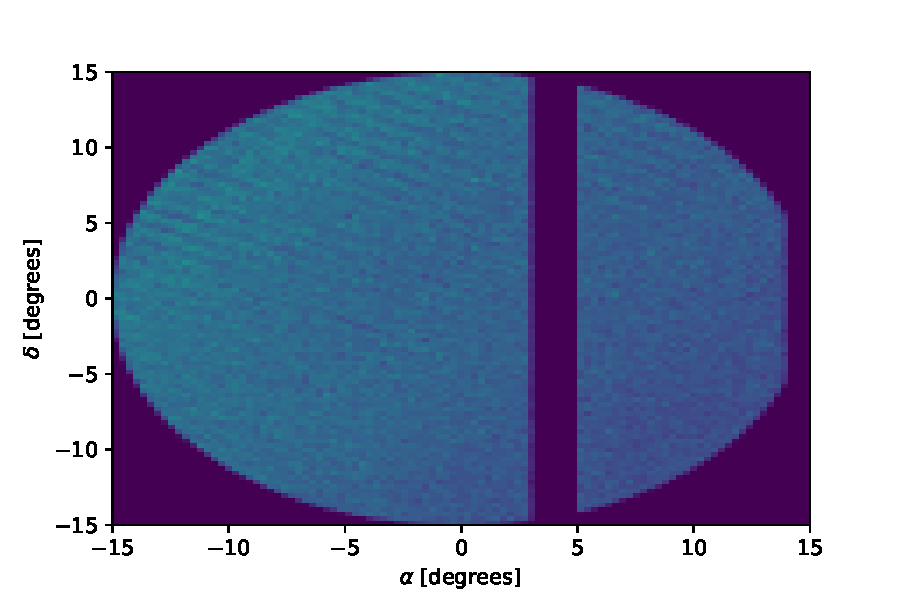
\includegraphics[width=0.5\textwidth]{../figures/histogram2dgaiascan_l337_5_b74_4_ra201_9_dec14_0_npy.pdf}\forloop{imagenum}{0}{\value{imagenum} < 18}{
\includegraphics[width=0.24\textwidth]{../figures/stars_passing_cut_rahistgaiascan_l337_5_b74_4_ra201_9_dec14_0_npy_\arabic{imagenum}.pdf}}
\caption{Region l$337.5$ b$74.4$ ra$201.9$ dec$14.0$}
\end{figure}

\begin{figure}[h!]
\centering
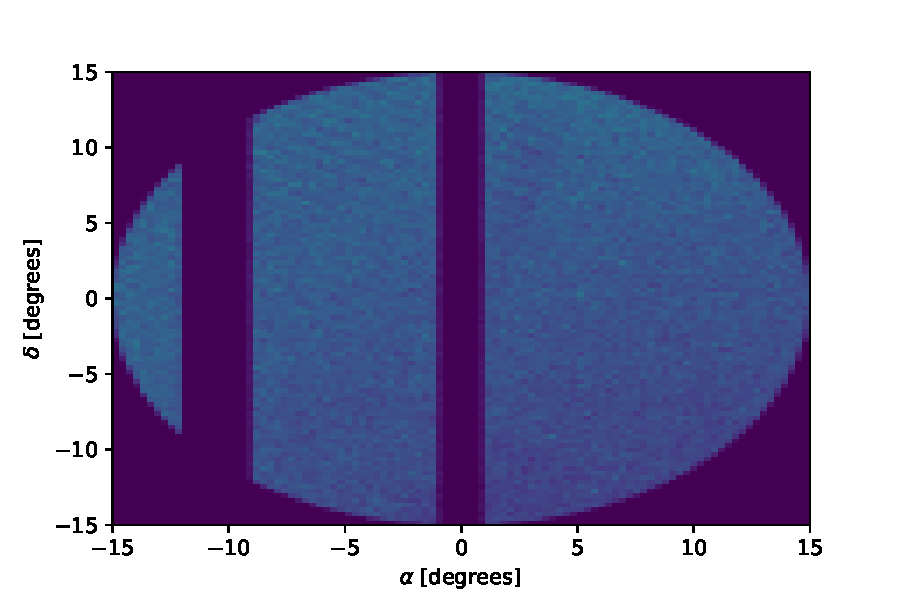
\includegraphics[width=0.5\textwidth]{../figures/histogram2dgaiascan_l45_0_b82_2_ra201_5_dec28_5_npy.pdf}\forloop{imagenum}{0}{\value{imagenum} < 17}{
\includegraphics[width=0.24\textwidth]{../figures/scanning_plotsgaiascan_l45_0_b82_2_ra201_5_dec28_5_npy_\arabic{imagenum}.pdf}}
\caption{Region l$45.0$ b$82.2$ ra$201.5$ dec$28.5$}
\end{figure}

\begin{figure}[h!]
\centering
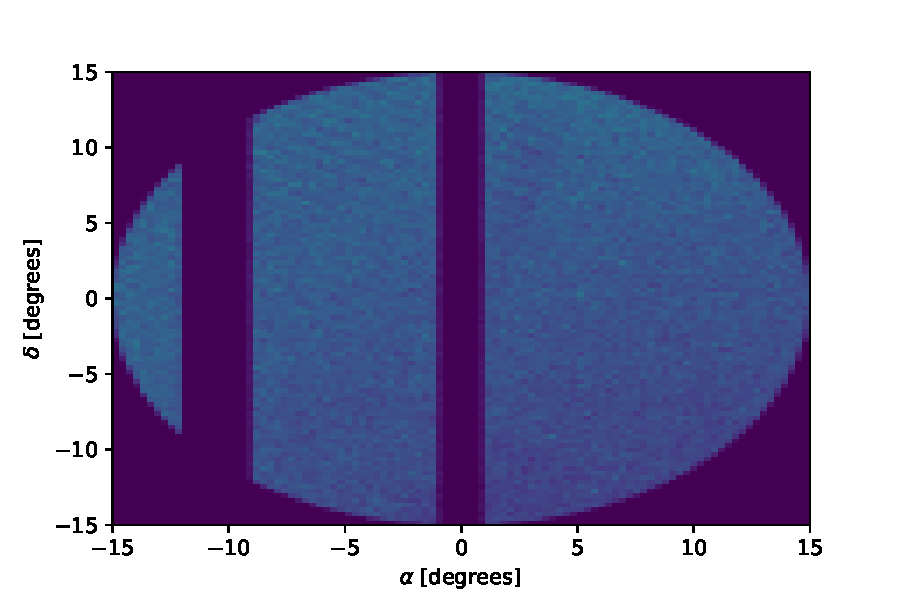
\includegraphics[width=0.5\textwidth]{../figures/histogram2dgaiascan_l45_0_b82_2_ra201_5_dec28_5_npy.pdf}\forloop{imagenum}{0}{\value{imagenum} < 17}{
\includegraphics[width=0.24\textwidth]{../figures/stars_near_zero_2dhistgaiascan_l45_0_b82_2_ra201_5_dec28_5_npy_\arabic{imagenum}.pdf}}
\caption{Region l$45.0$ b$82.2$ ra$201.5$ dec$28.5$}
\end{figure}

\begin{figure}[h!]
\centering
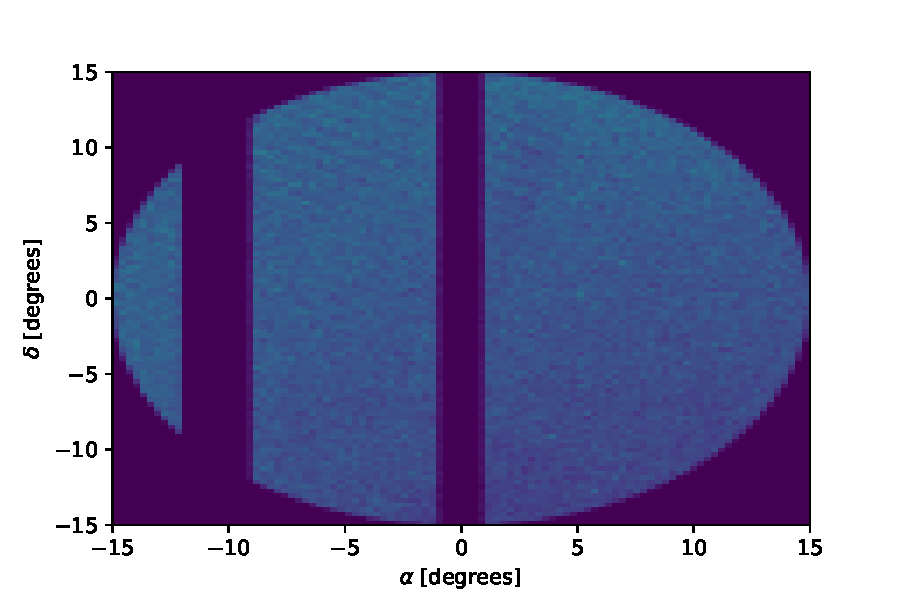
\includegraphics[width=0.5\textwidth]{../figures/histogram2dgaiascan_l45_0_b82_2_ra201_5_dec28_5_npy.pdf}\forloop{imagenum}{0}{\value{imagenum} < 17}{
\includegraphics[width=0.24\textwidth]{../figures/stars_near_zero_rahistgaiascan_l45_0_b82_2_ra201_5_dec28_5_npy_\arabic{imagenum}.pdf}}
\caption{Region l$45.0$ b$82.2$ ra$201.5$ dec$28.5$}
\end{figure}

\begin{figure}[h!]
\centering
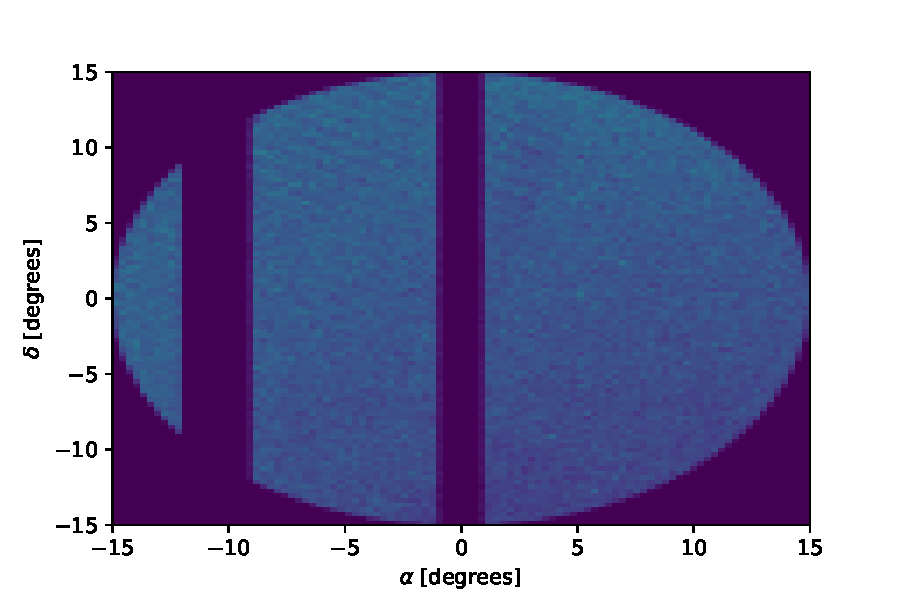
\includegraphics[width=0.5\textwidth]{../figures/histogram2dgaiascan_l45_0_b82_2_ra201_5_dec28_5_npy.pdf}\forloop{imagenum}{0}{\value{imagenum} < 17}{
\includegraphics[width=0.24\textwidth]{../figures/stars_passing_cutgaiascan_l45_0_b82_2_ra201_5_dec28_5_npy_\arabic{imagenum}.pdf}}
\caption{Region l$45.0$ b$82.2$ ra$201.5$ dec$28.5$}
\end{figure}

\begin{figure}[h!]
\centering
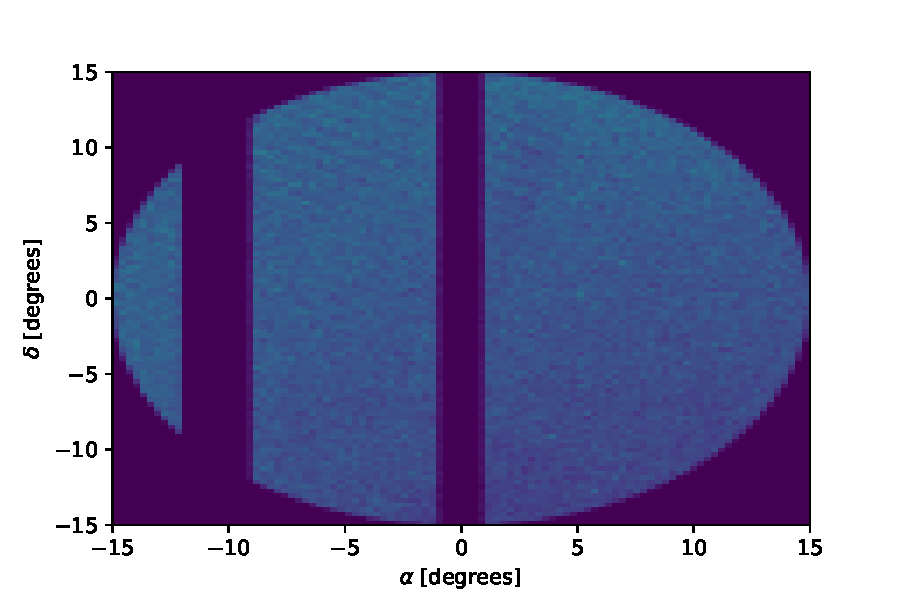
\includegraphics[width=0.5\textwidth]{../figures/histogram2dgaiascan_l45_0_b82_2_ra201_5_dec28_5_npy.pdf}\forloop{imagenum}{0}{\value{imagenum} < 17}{
\includegraphics[width=0.24\textwidth]{../figures/stars_passing_cut_rahistgaiascan_l45_0_b82_2_ra201_5_dec28_5_npy_\arabic{imagenum}.pdf}}
\caption{Region l$45.0$ b$82.2$ ra$201.5$ dec$28.5$}
\end{figure}

\begin{figure}[h!]
\centering
\includegraphics[width=0.5\textwidth]{../figures/histogram2dgaiascan_l67_5_b74_4_ra208_6_dec35_1_npy.pdf}\forloop{imagenum}{0}{\value{imagenum} < 18}{
\includegraphics[width=0.24\textwidth]{../figures/scanning_plotsgaiascan_l67_5_b74_4_ra208_6_dec35_1_npy_\arabic{imagenum}.pdf}}
\caption{Region l$67.5$ b$74.4$ ra$208.6$ dec$35.1$}
\end{figure}

\begin{figure}[h!]
\centering
\includegraphics[width=0.5\textwidth]{../figures/histogram2dgaiascan_l67_5_b74_4_ra208_6_dec35_1_npy.pdf}\forloop{imagenum}{0}{\value{imagenum} < 18}{
\includegraphics[width=0.24\textwidth]{../figures/stars_near_zero_2dhistgaiascan_l67_5_b74_4_ra208_6_dec35_1_npy_\arabic{imagenum}.pdf}}
\caption{Region l$67.5$ b$74.4$ ra$208.6$ dec$35.1$}
\end{figure}

\begin{figure}[h!]
\centering
\includegraphics[width=0.5\textwidth]{../figures/histogram2dgaiascan_l67_5_b74_4_ra208_6_dec35_1_npy.pdf}\forloop{imagenum}{0}{\value{imagenum} < 18}{
\includegraphics[width=0.24\textwidth]{../figures/stars_near_zero_rahistgaiascan_l67_5_b74_4_ra208_6_dec35_1_npy_\arabic{imagenum}.pdf}}
\caption{Region l$67.5$ b$74.4$ ra$208.6$ dec$35.1$}
\end{figure}

\begin{figure}[h!]
\centering
\includegraphics[width=0.5\textwidth]{../figures/histogram2dgaiascan_l67_5_b74_4_ra208_6_dec35_1_npy.pdf}\forloop{imagenum}{0}{\value{imagenum} < 18}{
\includegraphics[width=0.24\textwidth]{../figures/stars_passing_cutgaiascan_l67_5_b74_4_ra208_6_dec35_1_npy_\arabic{imagenum}.pdf}}
\caption{Region l$67.5$ b$74.4$ ra$208.6$ dec$35.1$}
\end{figure}

\begin{figure}[h!]
\centering
\includegraphics[width=0.5\textwidth]{../figures/histogram2dgaiascan_l67_5_b74_4_ra208_6_dec35_1_npy.pdf}\forloop{imagenum}{0}{\value{imagenum} < 18}{
\includegraphics[width=0.24\textwidth]{../figures/stars_passing_cut_rahistgaiascan_l67_5_b74_4_ra208_6_dec35_1_npy_\arabic{imagenum}.pdf}}
\caption{Region l$67.5$ b$74.4$ ra$208.6$ dec$35.1$}
\end{figure}

\begin{figure}[h!]
\centering
\includegraphics[width=0.5\textwidth]{../figures/histogram2dgaiascan_l75_0_b66_4_ra216_0_dec41_0_npy.pdf}\forloop{imagenum}{0}{\value{imagenum} < 18}{
\includegraphics[width=0.24\textwidth]{../figures/scanning_plotsgaiascan_l75_0_b66_4_ra216_0_dec41_0_npy_\arabic{imagenum}.pdf}}
\caption{Region l$75.0$ b$66.4$ ra$216.0$ dec$41.0$}
\end{figure}

\begin{figure}[h!]
\centering
\includegraphics[width=0.5\textwidth]{../figures/histogram2dgaiascan_l75_0_b66_4_ra216_0_dec41_0_npy.pdf}\forloop{imagenum}{0}{\value{imagenum} < 18}{
\includegraphics[width=0.24\textwidth]{../figures/stars_near_zero_2dhistgaiascan_l75_0_b66_4_ra216_0_dec41_0_npy_\arabic{imagenum}.pdf}}
\caption{Region l$75.0$ b$66.4$ ra$216.0$ dec$41.0$}
\end{figure}

\begin{figure}[h!]
\centering
\includegraphics[width=0.5\textwidth]{../figures/histogram2dgaiascan_l75_0_b66_4_ra216_0_dec41_0_npy.pdf}\forloop{imagenum}{0}{\value{imagenum} < 18}{
\includegraphics[width=0.24\textwidth]{../figures/stars_near_zero_rahistgaiascan_l75_0_b66_4_ra216_0_dec41_0_npy_\arabic{imagenum}.pdf}}
\caption{Region l$75.0$ b$66.4$ ra$216.0$ dec$41.0$}
\end{figure}

\begin{figure}[h!]
\centering
\includegraphics[width=0.5\textwidth]{../figures/histogram2dgaiascan_l75_0_b66_4_ra216_0_dec41_0_npy.pdf}\forloop{imagenum}{0}{\value{imagenum} < 18}{
\includegraphics[width=0.24\textwidth]{../figures/stars_passing_cutgaiascan_l75_0_b66_4_ra216_0_dec41_0_npy_\arabic{imagenum}.pdf}}
\caption{Region l$75.0$ b$66.4$ ra$216.0$ dec$41.0$}
\end{figure}

\begin{figure}[h!]
\centering
\includegraphics[width=0.5\textwidth]{../figures/histogram2dgaiascan_l75_0_b66_4_ra216_0_dec41_0_npy.pdf}\forloop{imagenum}{0}{\value{imagenum} < 18}{
\includegraphics[width=0.24\textwidth]{../figures/stars_passing_cut_rahistgaiascan_l75_0_b66_4_ra216_0_dec41_0_npy_\arabic{imagenum}.pdf}}
\caption{Region l$75.0$ b$66.4$ ra$216.0$ dec$41.0$}
\end{figure}

\begin{figure}[h!]
\centering
\includegraphics[width=0.5\textwidth]{../figures/histogram2dgaiascan_l78_8_b58_4_ra224_7_dec46_3_npy.pdf}\forloop{imagenum}{0}{\value{imagenum} < 18}{
\includegraphics[width=0.24\textwidth]{../figures/scanning_plotsgaiascan_l78_8_b58_4_ra224_7_dec46_3_npy_\arabic{imagenum}.pdf}}
\caption{Region l$78.8$ b$58.4$ ra$224.7$ dec$46.3$}
\end{figure}

\begin{figure}[h!]
\centering
\includegraphics[width=0.5\textwidth]{../figures/histogram2dgaiascan_l78_8_b58_4_ra224_7_dec46_3_npy.pdf}\forloop{imagenum}{0}{\value{imagenum} < 18}{
\includegraphics[width=0.24\textwidth]{../figures/stars_near_zero_2dhistgaiascan_l78_8_b58_4_ra224_7_dec46_3_npy_\arabic{imagenum}.pdf}}
\caption{Region l$78.8$ b$58.4$ ra$224.7$ dec$46.3$}
\end{figure}

\begin{figure}[h!]
\centering
\includegraphics[width=0.5\textwidth]{../figures/histogram2dgaiascan_l78_8_b58_4_ra224_7_dec46_3_npy.pdf}\forloop{imagenum}{0}{\value{imagenum} < 18}{
\includegraphics[width=0.24\textwidth]{../figures/stars_near_zero_rahistgaiascan_l78_8_b58_4_ra224_7_dec46_3_npy_\arabic{imagenum}.pdf}}
\caption{Region l$78.8$ b$58.4$ ra$224.7$ dec$46.3$}
\end{figure}

\begin{figure}[h!]
\centering
\includegraphics[width=0.5\textwidth]{../figures/histogram2dgaiascan_l78_8_b58_4_ra224_7_dec46_3_npy.pdf}\forloop{imagenum}{0}{\value{imagenum} < 18}{
\includegraphics[width=0.24\textwidth]{../figures/stars_passing_cutgaiascan_l78_8_b58_4_ra224_7_dec46_3_npy_\arabic{imagenum}.pdf}}
\caption{Region l$78.8$ b$58.4$ ra$224.7$ dec$46.3$}
\end{figure}

\begin{figure}[h!]
\centering
\includegraphics[width=0.5\textwidth]{../figures/histogram2dgaiascan_l78_8_b58_4_ra224_7_dec46_3_npy.pdf}\forloop{imagenum}{0}{\value{imagenum} < 18}{
\includegraphics[width=0.24\textwidth]{../figures/stars_passing_cut_rahistgaiascan_l78_8_b58_4_ra224_7_dec46_3_npy_\arabic{imagenum}.pdf}}
\caption{Region l$78.8$ b$58.4$ ra$224.7$ dec$46.3$}
\end{figure}

\begin{figure}[h!]
\centering
\includegraphics[width=0.5\textwidth]{../figures/histogram2dgaiascan_l99_0_b50_2_ra224_7_dec60_6_npy.pdf}\forloop{imagenum}{0}{\value{imagenum} < 18}{
\includegraphics[width=0.24\textwidth]{../figures/scanning_plotsgaiascan_l99_0_b50_2_ra224_7_dec60_6_npy_\arabic{imagenum}.pdf}}
\caption{Region l$99.0$ b$50.2$ ra$224.7$ dec$60.6$}
\end{figure}

\begin{figure}[h!]
\centering
\includegraphics[width=0.5\textwidth]{../figures/histogram2dgaiascan_l99_0_b50_2_ra224_7_dec60_6_npy.pdf}\forloop{imagenum}{0}{\value{imagenum} < 18}{
\includegraphics[width=0.24\textwidth]{../figures/stars_near_zero_2dhistgaiascan_l99_0_b50_2_ra224_7_dec60_6_npy_\arabic{imagenum}.pdf}}
\caption{Region l$99.0$ b$50.2$ ra$224.7$ dec$60.6$}
\end{figure}

\begin{figure}[h!]
\centering
\includegraphics[width=0.5\textwidth]{../figures/histogram2dgaiascan_l99_0_b50_2_ra224_7_dec60_6_npy.pdf}\forloop{imagenum}{0}{\value{imagenum} < 18}{
\includegraphics[width=0.24\textwidth]{../figures/stars_near_zero_rahistgaiascan_l99_0_b50_2_ra224_7_dec60_6_npy_\arabic{imagenum}.pdf}}
\caption{Region l$99.0$ b$50.2$ ra$224.7$ dec$60.6$}
\end{figure}

\begin{figure}[h!]
\centering
\includegraphics[width=0.5\textwidth]{../figures/histogram2dgaiascan_l99_0_b50_2_ra224_7_dec60_6_npy.pdf}\forloop{imagenum}{0}{\value{imagenum} < 18}{
\includegraphics[width=0.24\textwidth]{../figures/stars_passing_cutgaiascan_l99_0_b50_2_ra224_7_dec60_6_npy_\arabic{imagenum}.pdf}}
\caption{Region l$99.0$ b$50.2$ ra$224.7$ dec$60.6$}
\end{figure}

\begin{figure}[h!]
\centering
\includegraphics[width=0.5\textwidth]{../figures/histogram2dgaiascan_l99_0_b50_2_ra224_7_dec60_6_npy.pdf}\forloop{imagenum}{0}{\value{imagenum} < 18}{
\includegraphics[width=0.24\textwidth]{../figures/stars_passing_cut_rahistgaiascan_l99_0_b50_2_ra224_7_dec60_6_npy_\arabic{imagenum}.pdf}}
\caption{Region l$99.0$ b$50.2$ ra$224.7$ dec$60.6$}
\end{figure}

%===================================================================
\section{Conclusions} \label{sec:conclusions}
%===================================================================


%===================================================================
\section*{\label{sec::acknowledgments}Acknowledgments}
%===================================================================

This work was supported by the Department of Energy, Office of Science under contract number DE-AC02-05CH11231 and many more...

\bibliography{refs,HEPML}
\bibliographystyle{utphys}


\end{document}
